\documentclass{article}

\usepackage{xcolor}
\usepackage{amsmath}
\usepackage{enumitem}
\usepackage{graphicx}
\usepackage{hyperref}
\usepackage{geometry}
\usepackage{tikz}
\usepackage{pgfplots}
\usepackage{subcaption}
\usepackage{xepersian}

\settextfont{XB Kayhan}
% \setmathdigitfont{Yas}
\setlatintextfont{Times Newer Roman}

\title{\vspace{-4cm} \textbf{پاسخ تمرینات سری سوم درس شناسایی آماری الگو}}
\author{محمدرضا غفرانی  ۴۰۰۱۳۱۰۷۶}
\date{\today}

\usetikzlibrary{patterns}

\begin{document}

\maketitle

\section*{سوال یک}

\subsection*{قسمت الف}

نمودار هیستوگرام داده‌ها در شکل \ref{histogram} نمایش داده شده است.

\begin{figure}[h]
    \centering
    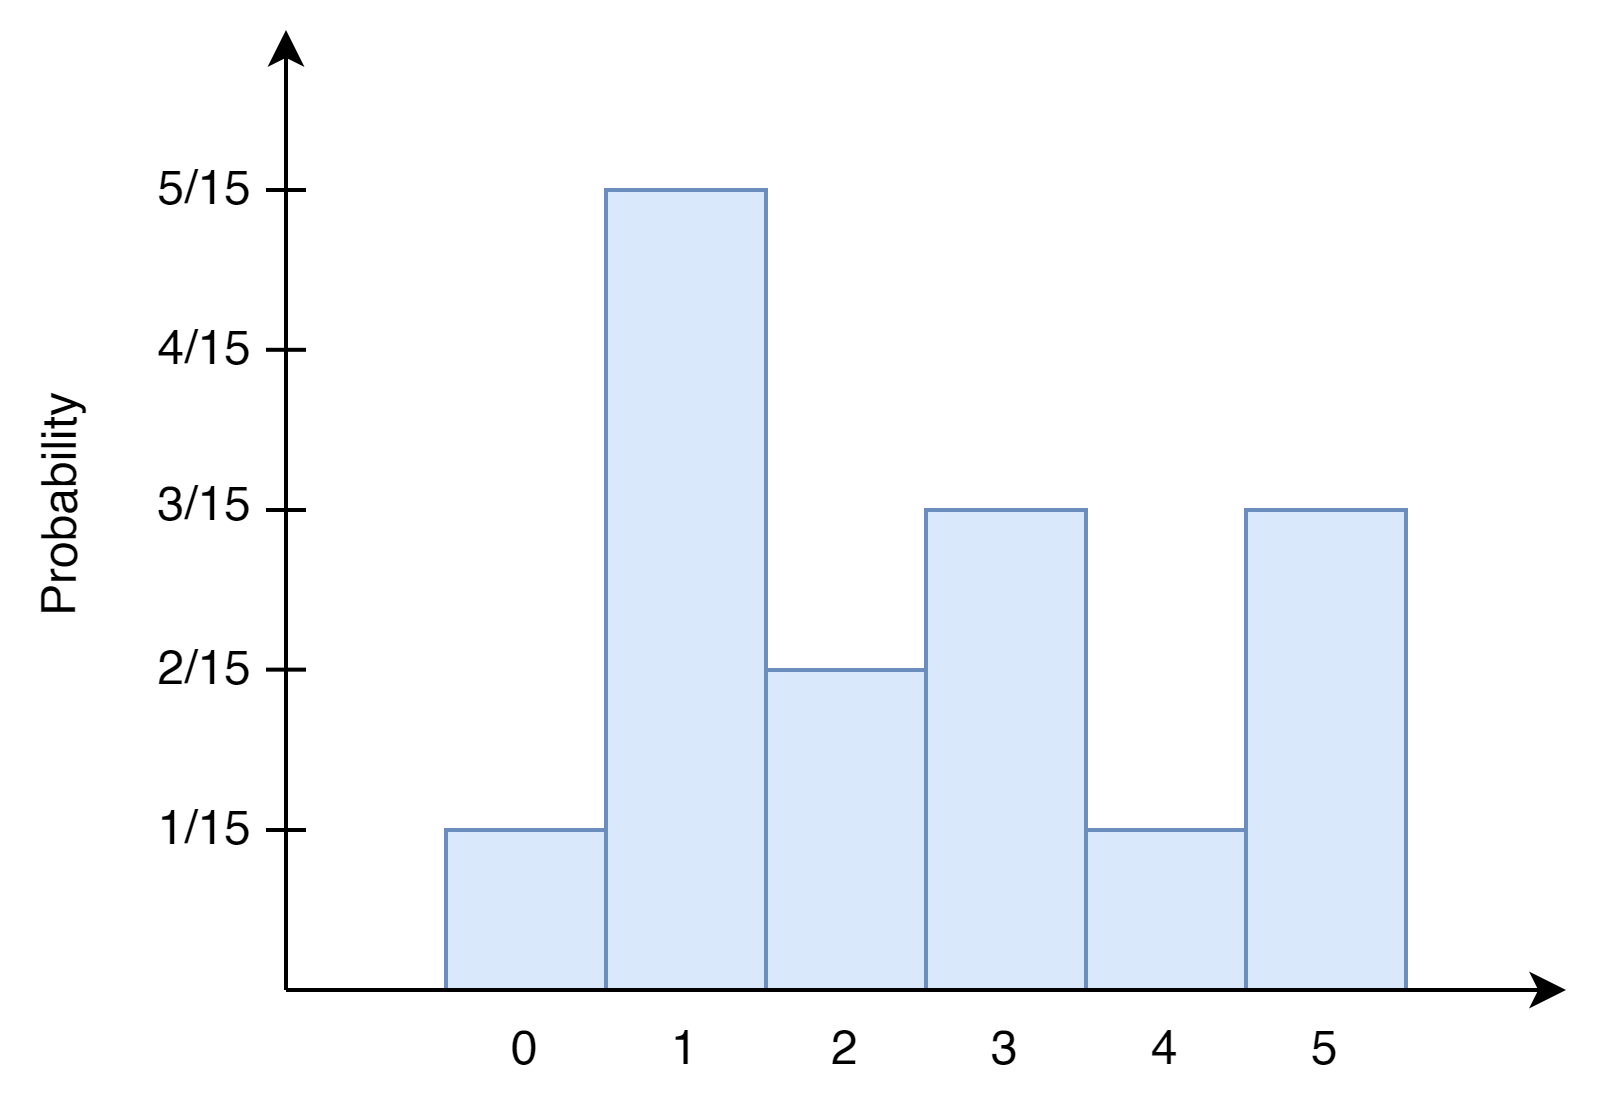
\includegraphics[scale=0.5]{images/q1/histogram.png}
    \caption{هیستوگرام داده‌های قسمت الف سوال یک}
    \label{histogram}
\end{figure}

\subsection*{قسمت ب}

در ادامه تخمینی که روش \lr{Parzen} به ازای هر $h$ داده شده می‌دهد، نمایش داده
شده است. (شکل \ref{parzen})

\begin{figure}[h]
    \begin{subfigure}{0.3\linewidth}
        \centering
        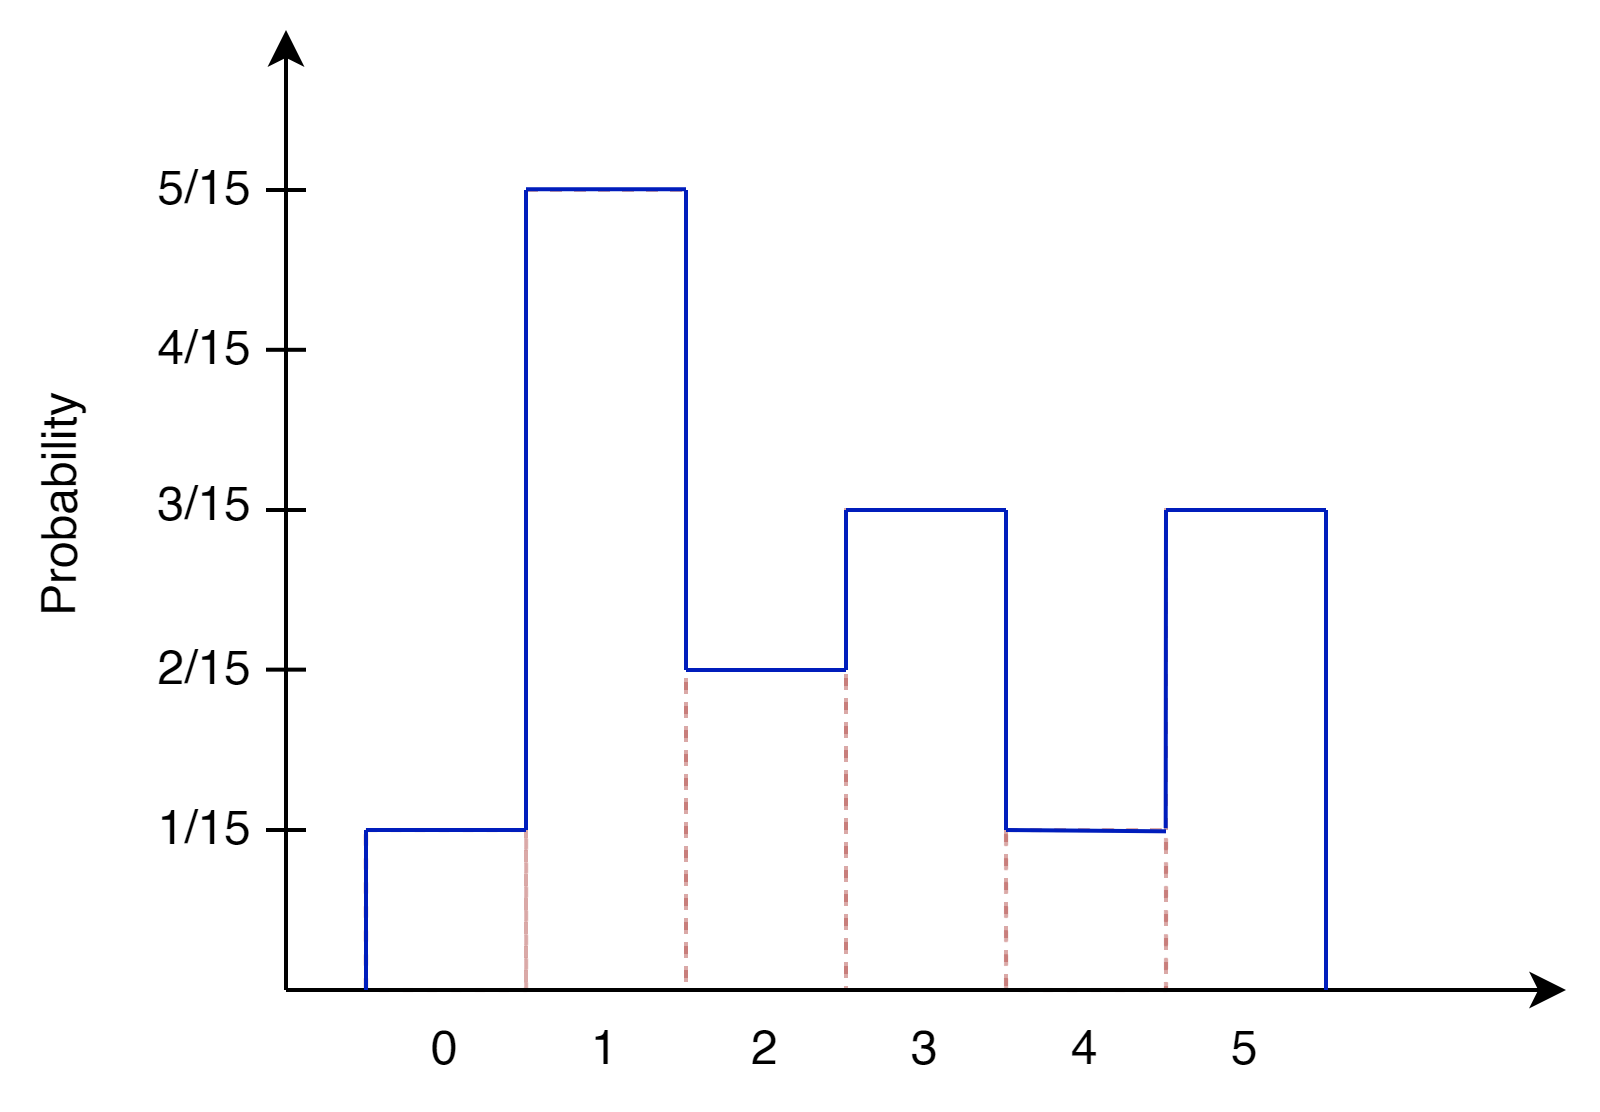
\includegraphics[width=\linewidth]{images/q1/parzen_h1.png}
        \caption{$h=1$}
    \end{subfigure}
    \hfill
    \begin{subfigure}{0.3\linewidth}
        \centering
        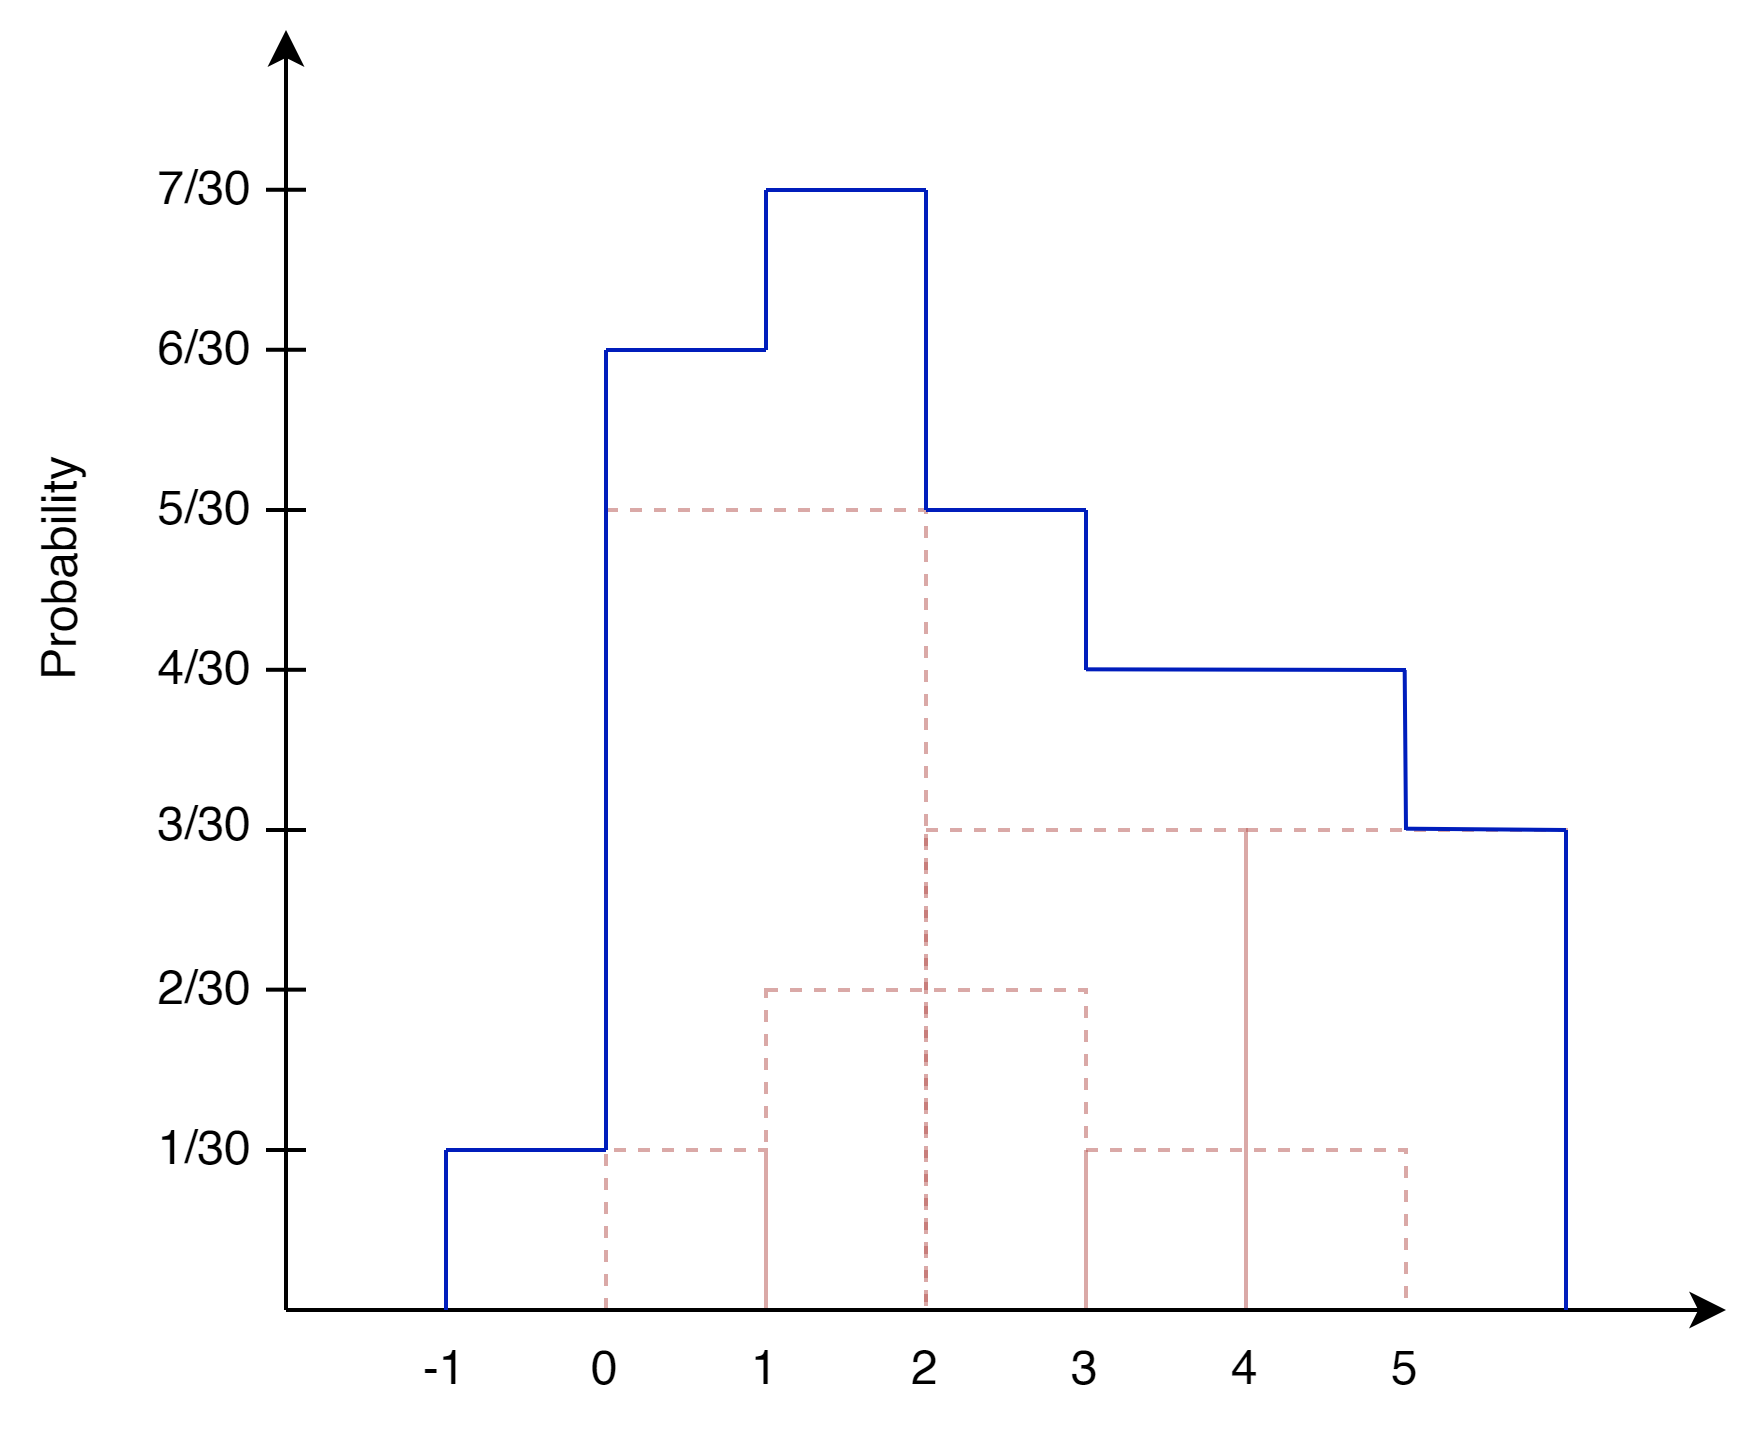
\includegraphics[width=\linewidth]{images/q1/parzen_h2.png}
        \caption{$h=2$}
    \end{subfigure}
    \hfill
    \begin{subfigure}{0.3\linewidth}
        \centering
        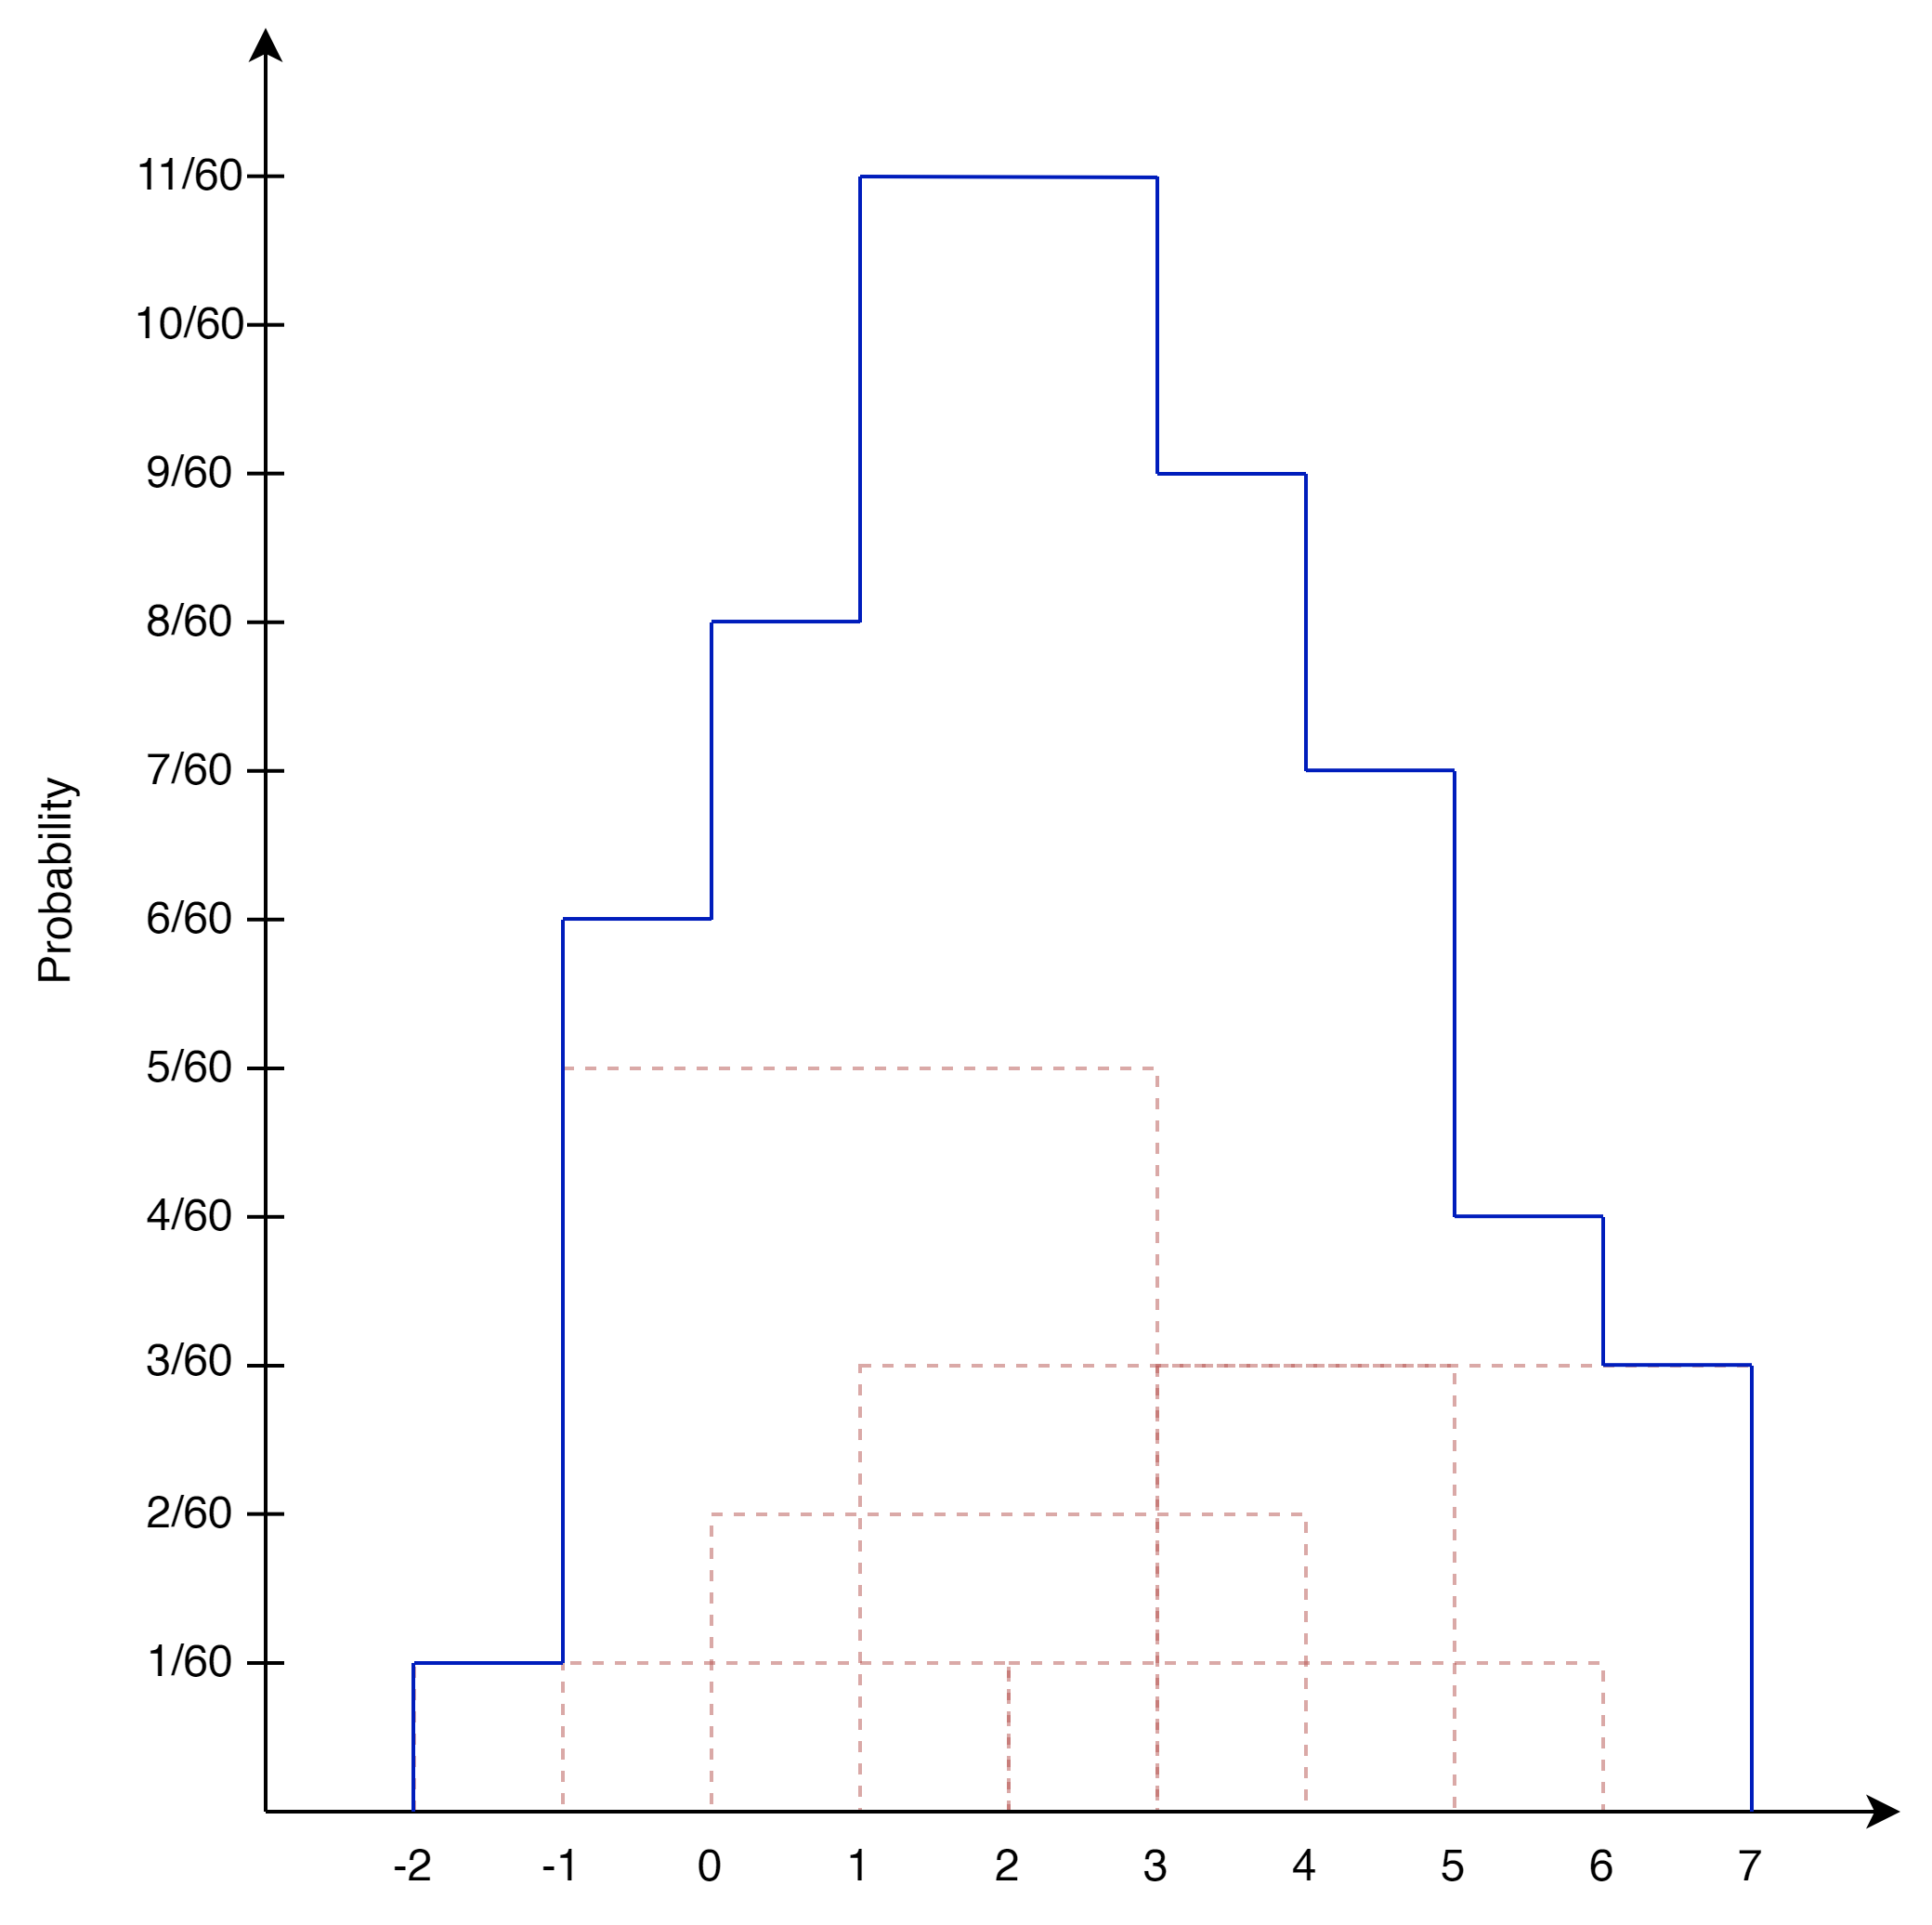
\includegraphics[width=\linewidth]{images/q1/parzen_h4.png}
        \caption{$h=4$}
    \end{subfigure}
    \caption{نمودار تخمین توزیع داده‌ها با استفاده از روش \lr{Parzen}}
    \label{parzen}
\end{figure}

\newpage

\subsection*{قسمت ج}

\begin{figure}[h]
    \centering
    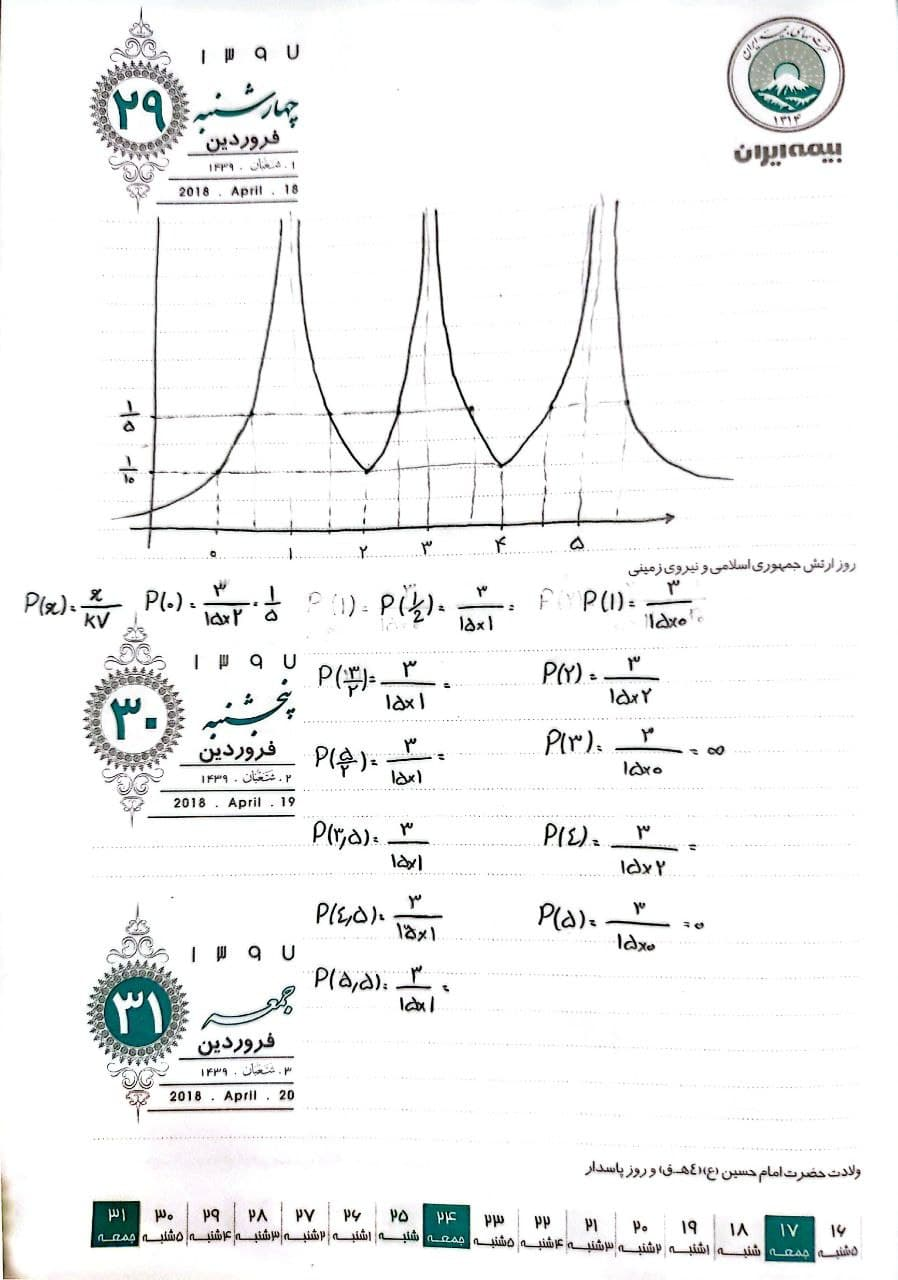
\includegraphics[scale=0.3]{images/q1/knn.jpg}
\end{figure}

\newpage

\subsection*{قسمت د}

می‌دانیم.

$$p(x) = \frac{1}{Nh^d}\sum_{i=1}^{N}K(u)$$

فرمول ریاضی تابع تخمین توزیع با استفاده از کرنل داده شده به صورت زیر حاصل می‌شود.

\begin{eqnarray*}
    p(x) = \frac{1}{15 \times 2^1}\Bigl(1 \times (1-|\frac{x-0}{2}|)\sigma(|\frac{x-0}{2}|\leq 1) + 5 \times (1-|\frac{x-1}{2}|)\sigma(|\frac{x-1}{2}| \leq 1)+& \\
    2 \times (1-|\frac{x-2}{2}|)\sigma(|\frac{x-2}{2}| \leq 1) + 3 \times (1-|\frac{x-3}{2}|)\sigma(|\frac{x-3}{2}| \leq 1) + & \\
    1 \times (1-|\frac{x-4}{2}|)\sigma(|\frac{x-4}{2}| \leq 1) + 3 \times (1-|\frac{x-5}{2}|)\sigma(|\frac{x-5}{2}| \leq 1)\Bigr)
\end{eqnarray*}

بنابراین

\begin{eqnarray*}
    p(x=0) & = & \frac{1}{30} (1 + \frac{5}{2}) = \frac{7}{60} \\
    p(x=1) & = & \frac{1}{30} (\frac{1}{2} + 5 + \frac{2}{2}) = \frac{13}{60} \\
    p(x=2) & = & \frac{1}{30} (\frac{5}{2} + 2 + \frac{3}{2}) = \frac{12}{60} \\
    p(x=3) & = & \frac{1}{30} (\frac{2}{2} + 3 + \frac{1}{2}) = \frac{9}{60} \\
    p(x=4) & = & \frac{1}{30} (\frac{3}{2} + 1 + \frac{3}{2}) = \frac{8}{60} \\
    p(x=5) & = & \frac{1}{30} (\frac{1}{2} + 3 ) = \frac{7}{60} \\
\end{eqnarray*}

\subsection*{قسمت ه}

با توجه به تابع کرنل و مقدار $h$، تنها نقاط $3, 4, 5$ موثر هستند. همچنین کرنل داده شده
تنها بر اساس تعداد داده‌های اطراف یک نقطه، به نقطه مد نظر مقدار می‌دهد. بنابراین از آنجا که
تعداد داده در اطراف نقطه $y=4$ برابر $7$ بوده و وزن پایه برای نقطه برابر $\frac{1}{15 \times 4}$ است،
در نتیجه مقدار تابع توزیع در نقطه $y=4$ برابر خواهد شد با $\frac{5}{60}$.

با استدلالی مشابه پاراگراف قبل مقدار تابع در نقطه $y=10$ و $y=16$ به ترتیب
برابر $\frac{1}{60}$ و $\frac{5}{60}$ خواهد شد.

\subsection*{قسمت و}

خواهیم داشت.

\begin{eqnarray*}
    p(x=4) & = & \frac{1}{15 \times 4^1} \sum_{i=1}^{15} K(\frac{4-x_i}{4}) = \frac{1}{60} \times 2.913 = 0.048 \\
    p(x=10) & = & \frac{1}{15 \times 4^1} \sum_{i=1}^{15} K(\frac{10-x_i}{4}) = \frac{1}{60} \times 2.897 = 0.048 \\
    p(x=16) & = & \frac{1}{15 \times 4^1} \sum_{i=1}^{15} K(\frac{16-x_i}{4}) = \frac{1}{60} \times 2.741 = 0.045
\end{eqnarray*}

\section*{سوال دو}

\subsection*{قسمت الف}

میانگین نمونه‌های داده شده برابر است با:

$$\bar{X} = \begin{bmatrix}6.4\\ 4.6\\ 5.7\end{bmatrix}$$

\subsection*{قسمت ب}

خواهیم داشت.

$$X - \bar{X} = \begin{bmatrix}
-5.4 & -3.4 & -2.4 & -0.4 & 0.6 & 1.6 & 1.6 & 1.6 & 2.6 & 3.6 \\
-4.6 & -0.6 & -1.6 & 2.4 & -3.6 & 3.4 & -2.6 & 5.4 & 0.4 & 1.4 \\
-2.7 & 0.3 & 1.3 & -2.7 & -0.7 & 4.3 & -1.7 & -3.7 & 2.3 & 3.3
\end{bmatrix}$$

\subsection*{قسمت ج}

خواهیم داشت.

\begin{eqnarray*}
    \Sigma = \frac{1}{N-1} (X - \bar{X})(X - \bar{X})^T & = & \frac{1}{9} (X - \bar{X})(X - \bar{X})^T \\
    & = & \begin{bmatrix}
        8.26 & 4.84 & 3.02 \\
        4.84 & 10.26 & 1.2 \\
        3.02 & 1.2 & 7.56
    \end{bmatrix}
\end{eqnarray*}

با توجه به ماتریس کوواریانس، میزان تغییرات به ازای هر ویژگی بیشتر از میزان تغییرات دو ویژگی نسبت به هم
است، به بیان دیگر اضافه کردن ویژگی‌های جدید تاثیر زیادی در پخش کردن داده‌های در فضا و بیشتر کردن احتمال جداکردن آن‌ها
از هم نداشته است.

\subsection*{قسمت د}

خواهیم داشت.

\begin{eqnarray*}
    \begin{bmatrix}8.26 & 4.84 & 3.02\\4.84 & 10.26 & 1.2\\3.02 & 1.2 & 7.56\end{bmatrix}v - \lambda v = 0
\end{eqnarray*}

با محاسبه‌ی مقدار بالا خواهیم داشت.

\begin{eqnarray*}
    \lambda_1 \simeq 15.28 & \hspace{1cm} & v_1 = \begin{bmatrix}0.62\\ 0.69\\ 0.35\end{bmatrix}\\
    \lambda_2 \simeq 7.26 & \hspace{1cm} & v_2 = \begin{bmatrix}0.13\\ -0.54\\ 0.82\end{bmatrix}\\
    \lambda_3 \simeq 3.54 & \hspace{1cm} & v_3 = \begin{bmatrix}0.76\\ -0.47\\ -0.43\end{bmatrix}\\
\end{eqnarray*}

\subsection*{قسمت ه}

بردار‌های ویژه‌ای که در قسمت قبل پیدا شده است را می‌توان به عنوان پا‌یه‌های این فضا استفاده کرد. لازم به ذکر است که
اگر بخواهیم داده‌ها را به فضای یک بعدی و یا دوبعدی منتقل کنیم طبق روش \lr{PCA} می‌توانیم به ترتیب از
بردار‌های $v_1$ و $(v_1, v_2)$ استفاده کنیم.

$$v_1 = \begin{bmatrix}0.62\\ 0.76\\ 0.13\end{bmatrix} \hspace{1cm} v_2 = \begin{bmatrix}0.35\\ -0.43\\ 0.82\end{bmatrix} \hspace{1cm} v_3 = \begin{bmatrix}0.69\\ -0.47\\ -0.54\end{bmatrix}$$


\subsection*{قسمت و}

نمایش داده‌ها در این فضای جدید به شکل زیر به دست می‌آید.

\begin{eqnarray*}
    \begin{bmatrix}v_1& v_2& v_3\end{bmatrix}^T (X - \bar{X}) =
    \begin{bmatrix}
        -7.537 & -2.449 & -2.158 & 0.453 & -2.36 &  4.881 & -1.393 & 3.433 & 2.727 & 4.402\\
        -0.448 & 0.125 & 1.63 & -3.596 & 1.459 & 1.923 & 0.219 & -5.792 & 2.032 & 2.448 \\
        -0.779 & -2.449 & -1.643 & -0.273 & 2.472 & -2.256 & 3.197 & 0.269 & 0.802 & 0.659
    \end{bmatrix}
\end{eqnarray*}

اگر بخواهیم داده‌ها را به فضای یک بعدی منتقل کنیم.

\begin{eqnarray*}
    v_1^T (X - \bar{X}) & = & \begin{bmatrix}0.62& 0.76& 0.13\end{bmatrix} \begin{bmatrix}-5.4 & -3.4 & -2.4 & -0.4 & 0.6 & 1.6 & 1.6 & 1.6 & 2.6 & 3.6 \\ -4.6 & -0.6 & -1.6 & 2.4 & -3.6 & 3.4 & -2.6 & 5.4 & 0.4 & 1.4 \\ -2.7 & 0.3 & 1.3 & -2.7 & -0.7 & 4.3 & -1.7 & -3.7 & 2.3 & 3.3\end{bmatrix}\\
    & = & \begin{bmatrix}-7.537 & -2.449 & -2.158 & 0.453 & -2.36 & 4.881 & -1.393 & 3.433 & 2.727 & 4.402\end{bmatrix}
\end{eqnarray*}

اگر بخواهیم داده‌ها را به فضای دو بعدی منتقل کنیم.

\begin{eqnarray*}
    \begin{bmatrix}v_1& v_2\end{bmatrix}^T (X - \bar{X}) & = & \begin{bmatrix}0.62& 0.76& 0.13\\ 0.35& -0.43& 0.82\end{bmatrix} \begin{bmatrix}-5.4 & -3.4 & -2.4 & -0.4 & 0.6 & 1.6 & 1.6 & 1.6 & 2.6 & 3.6 \\ -4.6 & -0.6 & -1.6 & 2.4 & -3.6 & 3.4 & -2.6 & 5.4 & 0.4 & 1.4 \\ -2.7 & 0.3 & 1.3 & -2.7 & -0.7 & 4.3 & -1.7 & -3.7 & 2.3 & 3.3\end{bmatrix}\\
    & = & \begin{bmatrix}-7.537 & -2.449 & -2.158 & 0.453 & -2.36 &  4.881 & -1.393 & 3.433 & 2.727 & 4.402\\ -0.448 & 0.125 & 1.63 & -3.596 & 1.459 & 1.923 & 0.219 & -5.792 & 2.032 & 2.448 \\\end{bmatrix}
\end{eqnarray*}

\subsection*{قسمت ز}

خواهیم داشت.

$$\bar{w}_1 = \begin{bmatrix}4.9\\ 3.2\\ 5\end{bmatrix} \hspace{1cm} \bar{w}_2 = \begin{bmatrix}6\\ 8.1\\ 4.8\end{bmatrix}$$

\subsection*{قسمت ح}

خواهیم داشت.

$$\Sigma_1 = \frac{1}{n-1} (w_1 - \bar{w}_1) (w_1 - \bar{w}_1)^T = \begin{bmatrix}10.32 & 3.35 & -4.33\\ 3.35 & 3.06 & -2.77\\-4.33 & -2.77 & 8.66\end{bmatrix}$$
$$\Sigma_2 = \frac{1}{n-1} (w_2 - \bar{w}_2) (w_2 - \bar{w}_2)^T = \begin{bmatrix}7.11 & 1.66 & 1.88\\ 1.66 & 1.87 & 1.24\\ 1.88 & 1.24 & 12.84\end{bmatrix}$$

\subsection*{قسمت ط}

خواهیم داشت.

\begin{eqnarray*}
    S_w = S_1 + S_2 & = & (n_1-1)\Sigma_1 + (n_2-1)\Sigma_2 \\
    & = & 9 \Sigma_1 + 9 \Sigma_2 \\
    & = & \begin{bmatrix}156.9 & 45.2 & -22\\ 45.2 & 44.5 & -13.8\\ -22 & -13.8 & 193.6\end{bmatrix}
\end{eqnarray*}

\subsection*{قسمت ی}

داریم.

\begin{eqnarray*}
    S_b & = & (\bar{w}_1 - \bar{w}_2)(\bar{w}_1 - \bar{w}_2)^T \\
    & = & \begin{bmatrix}1.21 & 5.39 & -0.22\\ 5.39 & 24.01 & -0.98\\ -0.22 & -0.98 & 0.04\end{bmatrix}
\end{eqnarray*}

\subsection*{قسمت ک}

می‌دانیم بردار $v$ در \lr{LDA} با استفاده از فرمول $S_w^{-1} (\mu_1 - \mu_2)$ به دست می‌آید، بنابراین

\begin{eqnarray*}
    v & = & S_w^{-1} (\bar{w}_1 - \bar{w}_2) \\
    & = & \begin{bmatrix}0.009 & -0.009 & 0.0003\\ -0.009 & 0.032 & 0.001\\0.0003 & 0.001 & 0.005\end{bmatrix}(\begin{bmatrix}4.9\\ 3.2\\ 5\end{bmatrix} - \begin{bmatrix}6\\ 8.1\\ 4.8\end{bmatrix}) \\
    & = & \begin{bmatrix}0.034\\ -0.146\\ 0.005\end{bmatrix}
\end{eqnarray*}

\subsection*{قسمت ل}

خواهیم داشت.

\begin{eqnarray*}
    y_1 & = & v^Tw_1 \\
    & = &  \begin{bmatrix}-0.479 & -0.110 & -0.279 & -0.087 & -0.460 & -0.561 & -0.074 & -0.180 & -0.451 & -0.598 \end{bmatrix} \\
    y_2 & = & v^Tw_2 \\
    y_2 & = & \begin{bmatrix}-0.964 & -1.121 & -0.708 & -1.165 & -1.323 & -0.832 & -0.870 & -0.954 & -1.156 & -0.993 \end{bmatrix}
\end{eqnarray*}

\subsection*{قسمت م تا ص}

شکل‌های متناظر قسمت‌های م تا ص در شکل \ref{q2_m_to_r_figures} آورده شده است.

\begin{figure}[h]
    \begin{subfigure}{0.3\linewidth}
        \centering
        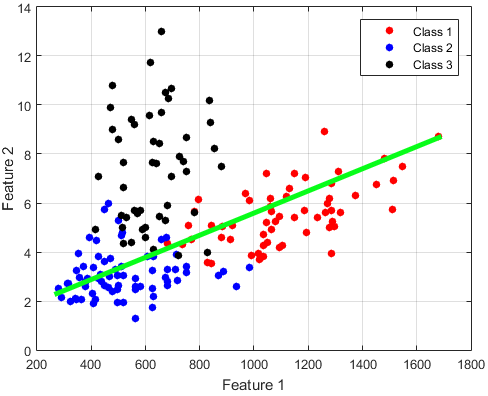
\includegraphics[scale=0.15]{images/q2/pca.png}
        \caption{عملکرد روش کاهش بعد \lr{PCA} با بر روی ویژگی‌های ۱ و ۲}
    \end{subfigure}
    \hfill
    \begin{subfigure}{0.3\linewidth}
        \centering
        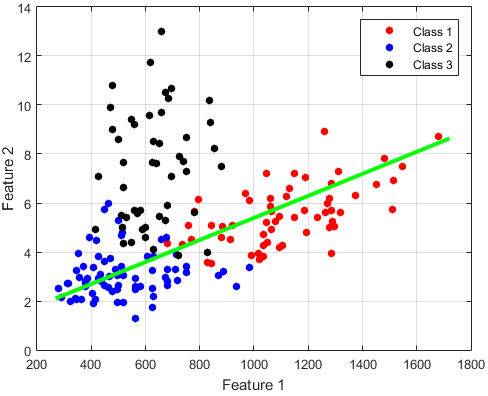
\includegraphics[scale=0.15]{images/q2/fisher.png}
        \caption{عملکرد روش کاهش بعد \lr{Fisher} با بر روی ویژگی‌های ۱ و ۲}
    \end{subfigure}
    \hfill
    \begin{subfigure}{0.3\linewidth}
        \centering
        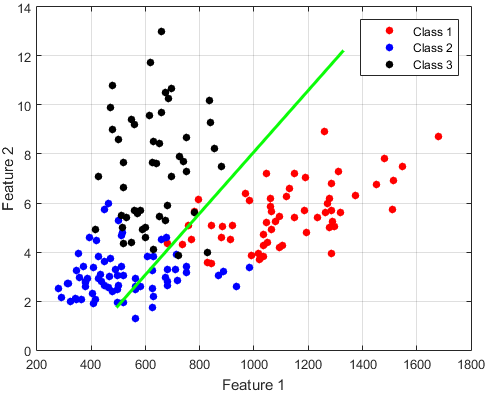
\includegraphics[scale=0.15]{images/q2/pca13.png}
        \caption{عملکرد روش کاهش بعد \lr{PCA} با بر روی ویژگی‌های ۱ و ۳}
    \end{subfigure}
    \newline
    \begin{subfigure}{0.3\linewidth}
        \centering
        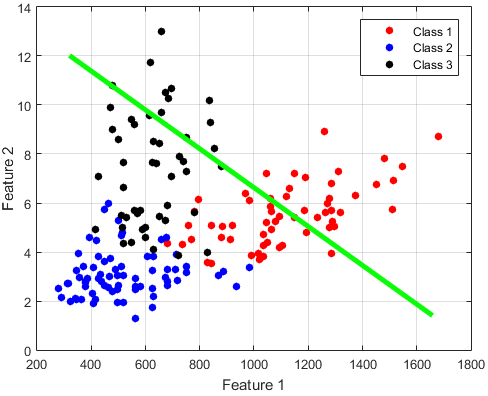
\includegraphics[scale=0.15]{images/q2/fisher13.png}
        \caption{عملکرد روش کاهش بعد \lr{Fisher} با بر روی ویژگی‌های ۱ و ۳}
    \end{subfigure}
    \hfill
    \begin{subfigure}{0.3\linewidth}
        \centering
        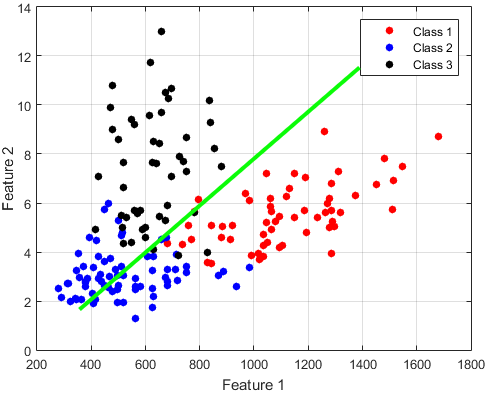
\includegraphics[scale=0.15]{images/q2/pca_all.png}
        \caption{عملکرد روش کاهش بعد \lr{PCA} با بر روی تمام ویژگی‌ها}
    \end{subfigure}
    \hfill
    \begin{subfigure}{0.3\linewidth}
        \centering
        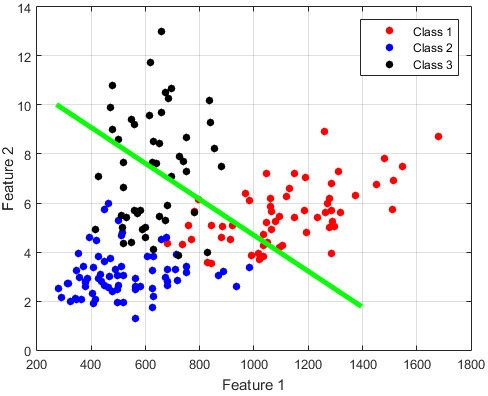
\includegraphics[scale=0.15]{images/q2/fisher_all.png}
        \caption{عملکرد روش کاهش بعد \lr{Fisher} با بر روی تمام ویژگی‌ها}
    \end{subfigure}
    \caption{شکل‌های متناظر قسمت م تا ص سوال ۲}
    \label{q2_m_to_r_figures}
\end{figure}

\section*{سوال سه}

لازم به ذکر است که برای انجام این سوال ستون‌های \lr{Date} و \lr{Location} حذف شده‌اند. چرا
که ماهیت این ستون‌ها به دسته‌بندی کمکی نمی‌کرد.

\subsection*{قسمت الف}

در شکل \ref{corr} بخشی از جدول ضرایب همبستگی بین هر زوج از ویژگی‌ها آورده شده است.
با بررسی دقیق این جدول متوجه می‌شویم که ضریب همبستگی بین دو ویژگی \lr{MaxTemp} و
\lr{Temp3pm} و همچنین بین دو ویژگی \lr{Pressure9am} و \lr{Pressure3pm} بیشتر از $0.95$ است.
در این جا ما ویژگی‌های \lr{MaxTemp} و \lr{Pressure9am} را حذف می‌کنیم.

نگه داشتن ویژگی‌هایی که ضریب همبستگی بین آن‌ها زیاد است، فایده‌ای ندارد. چرا که یکی از ویژگی‌ها
مقادیر بیان شده توسط ویژگی دیگر را نیز شامل می‌شود و در نتیجه نگه‌داشتن هر دو آن‌ها تنها باعث \lr{Overfitting}
و افزایش محاسبات ما می‌شود.

\begin{figure}[h]
    \centering
    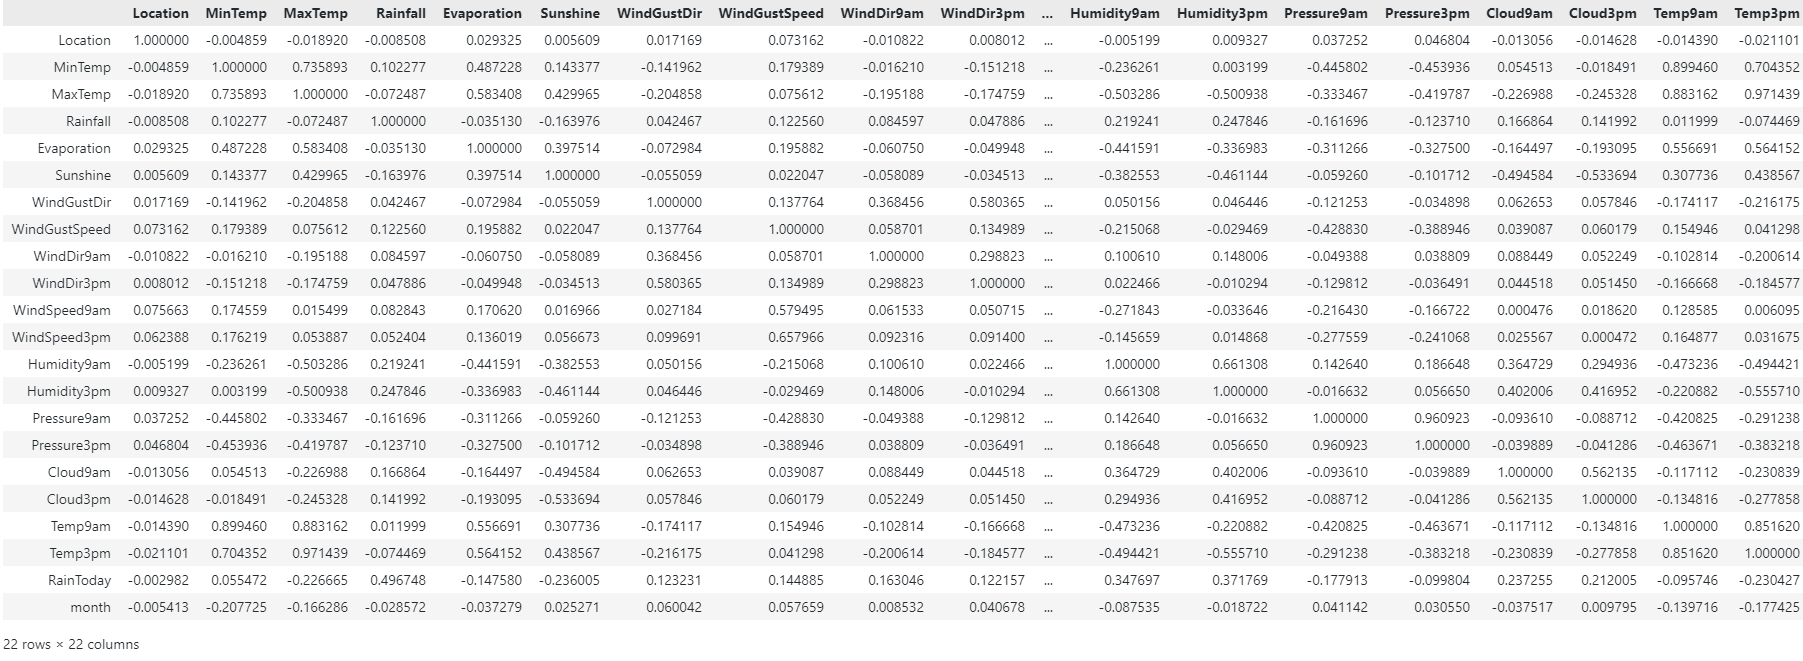
\includegraphics[width=0.7\linewidth]{images/q3/corr.png}
    \caption{ضرایب همبستگی بین زوج موجودیت‌ها در سوال سه}
    \label{corr}
\end{figure}

\subsection*{قسمت ب}

برای انجام این قسمت از تابع

\begin{center}
    \lr{\texttt{sklearn.feature\_selection.SequentialFeatureSelector}}
\end{center}

کمک می‌گیریم. این تابع که توسط کتابخانه \lr{scikit-learn} در اختیار ما قرار گرفته است. این تابع برای انجام
وظیفه خود نیاز به یک دسته‌بندی دارد. در این جا ما از دسته‌بند \lr{kNN} با مقدار
$k=3$ استفاده می‌کنیم. این دسته‌بند نیز توسط کتابخانه \lr{scikit-learn} توسعه داده شده است.
در نهایت با انجام روال انتخاب ویژگی‌ها به ویژگی‌های زیر می‌رسیم.

\begin{center}
    \begin{latin}
        MinTemp, Rainfall, Sunshine, WindGustDir, WindGustSpeed, WindDir3pm, \\
        WindSpeed3pm, Humidity3pm, Pressure3pm, Temp3pm
    \end{latin}
\end{center}

\subsection*{قسمت ج}

با امتحان کردن مقادیر مختلف برای $k$در بازه $[1,29]$ به نمودار \ref{accuracy_k} دست پیدا می‌کنیم.
با توجه به این نمودار به نظر می‌رسد بهترین مقدار برای $k$ مقدار 19 باشد چرا که
تا زمانی که $k<19$ است دقت الگوریتم شیب صعودی دارد. اما زمانی که مقدار $k$ از 19 فراتر می‌رود،
دقت الگوریتم تقریبا ثابت باقی می‌ماند. بنابراین اگر مقادیر بزرگتری را به عنوان $k$ انتخاب کنیم،
الگوریتم پیچیده‌تر شده و احتمال \lr{overfitting} بیشتر می‌شود.

\begin{figure}
    \centering
    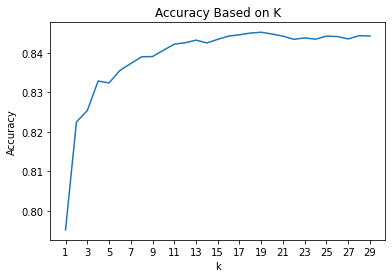
\includegraphics[width=0.7\linewidth]{images/q3/accuracy_k.png}
    \caption{دقت دسته‌بندی \lr{kNN} در به ازای $k$های مختلف}
    \label{accuracy_k}
\end{figure}

\subsection*{قسمت د}

برای انجام این قسمت از داده‌های روز دوشنبه مورخ ۱۷ ژانویه 2022 استفاده کرده‌ایم و سعی کرده‌ایم پیش‌بینی کنیم
که آیا در روز سه‌شنبه باران (=برف) خواهد بارید یا خیر. در شکل \ref{rasht}
صفحه‌ای که اطلاعات از آن استخراج شده مشاهده می‌شود.

\begin{figure}[h]
    \centering
    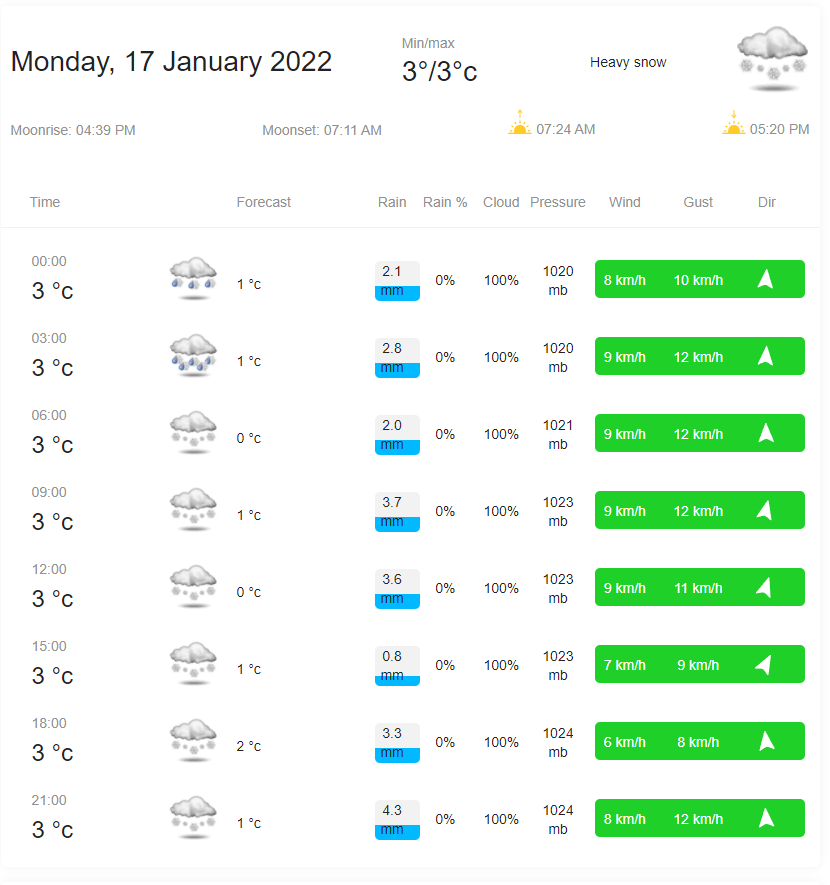
\includegraphics[scale=0.2]{images/q3/rasht.png}
    \caption{آب و هوای رشت در روز ۱۷ ژانویه ۲۰۲۲}
    \label{rasht}
\end{figure}

ما برای انجام دسته‌بندی تنها به مقادیر 10 ویژگی که پیشتر ذکر شد نیاز داریم، بنابراین سعی می‌کنیم
این مقادیر را به دست بیاریم. اکثر مقادیر به راحتی از جدول به دست می‌آید که در ادامه آورده شده‌اند.

\begin{latin}
    'MinTemp': 3 \\
    'Rainfall':22.6 \\
    'Sunshine': None \\
    'WindGustSpeed': 5 \\
    'WindGustDir': 10.75 \\
    'WindDir3pm': 4 \\
    'WindSpeed3pm': 7 \\
    'Humidity3pm': None \\
    'Pressure3pm': 1023 \\
    'Temp3pm': 3
\end{latin}

همان‌طور که مشاهده می‌شود، تنها برای دو مقدار \lr{Sunshine} و \lr{Humidity3pm} مقداری از جدول یافت نشده است.
مقادیر این دو ستون را نیز با توجه به مفهومی که از آن‌ها برداشت می‌شود، می‌توان تعیین کرد. با مطالعه منبع
\lr{BOM} در رابطه با معنی ستون \lr{Sunshine} به این نتیجه می‌رسیم که این ستون تعداد ساعت‌های آفتابی روز را
نشان می‌دهد. بنابراین در این جا با توجه به این که تمامی روز هوا برفی بوده است در نتیجه منطقی است که
تعداد ساعت‌های آفتابی صفر باشد. از طرف دیگر با توجه به آن که در ساعت ۳ بعد از هوا برفی بوده است
در نتیجه می‌توان جمله را بیان کرد که رطوبت هوا 100\% است.

در نهایت با انجام همه‌ی این عملیات مدل پیش‌بینی کرد که فردا یعنی روز سه‌شنبه باران خواهد بارید. با
بررسی در سایت متوجه می‌شویم که در روز سه‌شنبه در ساعات اولیه در حد $0.1$ میلی‌متر باران خواهد بارید و
مدل اشتباه بزرگی نکرده است.

\subsection*{قسمت ه}

برای پیش‌بینی احتمال باریدن باران همچنان می‌توان از \lr{kNN} کمک گرفت. بدین شکل که
مثل قبل $k$ نزدیک‌ترین همسایه به نمونه فعلی را پیدا می‌کنیم و سپس به جای آن که
تعداد نمونه‌هایی که دلالت بر باریدن باران دارند را بشمریم و اگر تعداد آن‌ها
بیشتر بود، نمونه را به صورت قطعی در کلاس باریدن باران پیش‌بینی کنیم؛ تعداد نمونه‌هایی که دلالت
بر باریدن باران را دارند می‌شمریم و این مقدار را بر $k$ تقسیم می‌کنیم. عدد حاصل شده احتمال آن را
نشان می‌دهد که در روز مد نظر هوا بارانی باشد.

\section*{سوال چهار}

\subsection*{قسمت ب}

تصویر میانگین و تصاویر ۸ بردار ویژه متناظر با مقادیر ویژه بزرگ در شکل \ref{donald_eigen} دیده می‌شود.
به جهت جلوگیری از شلوغی بی‌مورد گزارش، بردار‌های متناظر مقادیر ویژه تنها در \lr{JupyterNotebook} متناظر
آورده شده است.

\begin{figure}[h]
    \begin{subfigure}{0.2\linewidth}
        \centering
    \end{subfigure}
    \hfill
    \begin{subfigure}{0.2\linewidth}
        \centering
        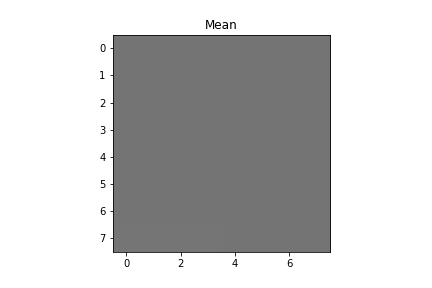
\includegraphics[scale=0.2]{images/q4/donald/mean.png}
    \end{subfigure}
    \hfill
    \begin{subfigure}{0.2\linewidth}
        \centering
    \end{subfigure}
    \newline
    \begin{subfigure}{0.2\linewidth}
        \centering
        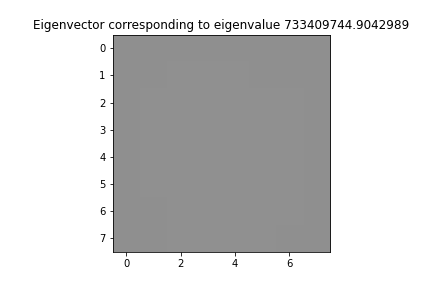
\includegraphics[scale=0.2]{images/q4/donald/eigenvector0.png}
    \end{subfigure}
    \hfill
    \begin{subfigure}{0.2\linewidth}
        \centering
        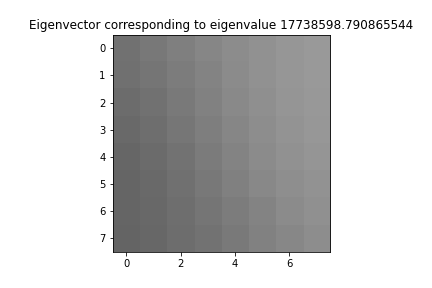
\includegraphics[scale=0.2]{images/q4/donald/eigenvector1.png}
    \end{subfigure}
    \hfill
    \begin{subfigure}{0.2\linewidth}
        \centering
        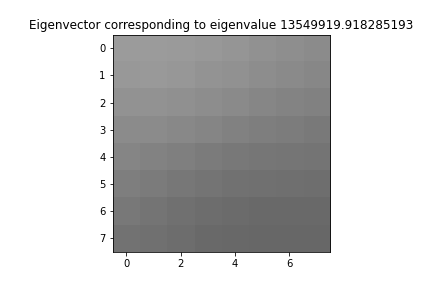
\includegraphics[scale=0.2]{images/q4/donald/eigenvector2.png}
    \end{subfigure}
    \hfill
    \begin{subfigure}{0.2\linewidth}
        \centering
        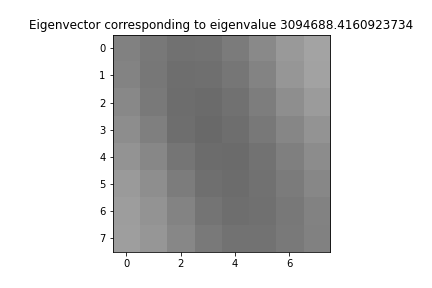
\includegraphics[scale=0.2]{images/q4/donald/eigenvector3.png}
    \end{subfigure}
    \newline
    \begin{subfigure}{0.2\linewidth}
        \centering
        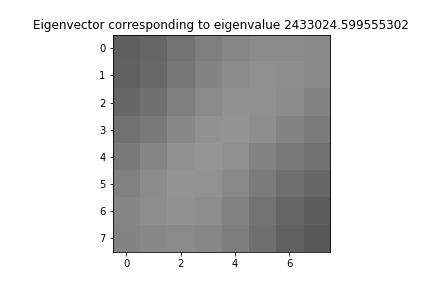
\includegraphics[scale=0.2]{images/q4/donald/eigenvector4.png}
    \end{subfigure}
    \hfill
    \begin{subfigure}{0.2\linewidth}
        \centering
        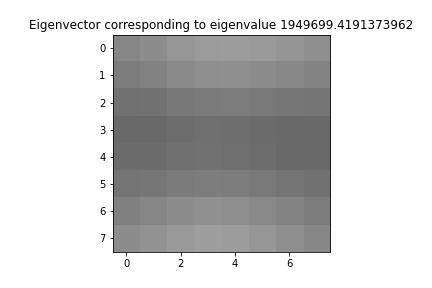
\includegraphics[scale=0.2]{images/q4/donald/eigenvector5.png}
    \end{subfigure}
    \hfill
    \begin{subfigure}{0.2\linewidth}
        \centering
        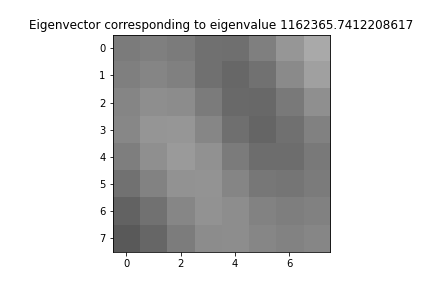
\includegraphics[scale=0.2]{images/q4/donald/eigenvector6.png}
    \end{subfigure}
    \hfill
    \begin{subfigure}{0.2\linewidth}
        \centering
        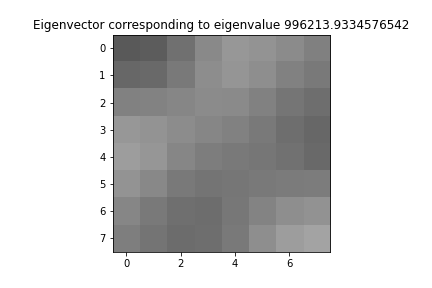
\includegraphics[scale=0.2]{images/q4/donald/eigenvector7.png}
    \end{subfigure}
    \caption{بردار‌های ویژه حاصل شده تصویر \lr{donald.jpg}}
    \label{donald_eigen}
\end{figure}

\subsection*{قسمت ه}

تصاویر به شکل زیر به دست می‌آید. (شکل \ref{donald}) همان‌طور که انتظار داریم با بیشتر شدن $k$ و افزایش تعداد بردار‌ ویژه‌های
دخیل ساخت تصویر، تصویر بازسازی شده از کیفیت بالاتری برخوردار است. هنگامی که مقدار پارامتر $k$ کم است صرفا کلیات تصویر
قابل شناسایی است اما با بیشتر شدن مقدار $k$ جزئیات تصویر کم‌کم نمایش داده می‌شود.

\begin{figure}[h]
    \begin{subfigure}{0.2\linewidth}
        \centering
        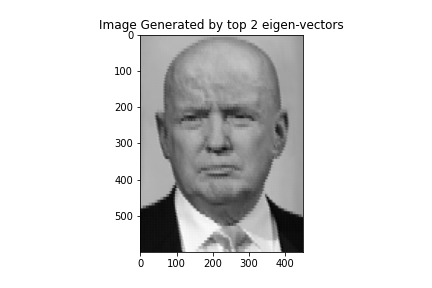
\includegraphics[scale=0.2]{images/q4/donald/donald_2.png}
    \end{subfigure}
    \hfill
    \begin{subfigure}{0.2\linewidth}
        \centering
        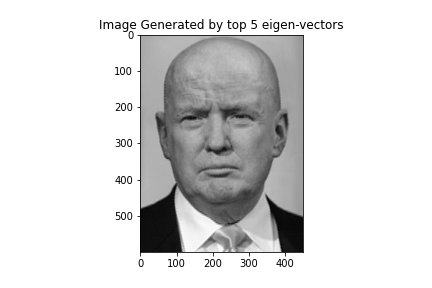
\includegraphics[scale=0.2]{images/q4/donald/donald_5.png}
    \end{subfigure}
    \hfill
    \begin{subfigure}{0.2\linewidth}
        \centering
        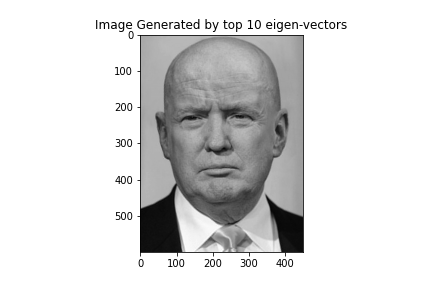
\includegraphics[scale=0.2]{images/q4/donald/donald_10.png}
    \end{subfigure}
    \hfill
    \begin{subfigure}{0.2\linewidth}
        \centering
        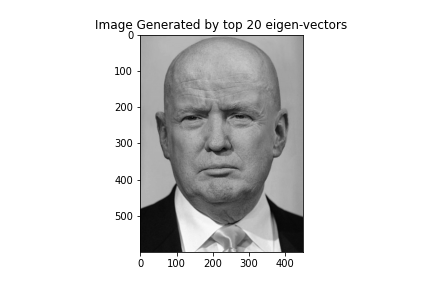
\includegraphics[scale=0.2]{images/q4/donald/donald_20.png}
    \end{subfigure}
    \caption{تصاویر ساخته بازسازی شده با استفاده از تصاویر ویژه}
    \label{donald}
\end{figure}

\subsection*{قسمت و}

برای عملیات بر روی این تصویر رنگی، ابتدا آن را به مولفه‌های سازنده‌اش یعنی مولفه قرمز، آبی و سبز می‌شکنیم. سپس
عملیات انجام شده برای تصویر \lr{donald.png} را تک‌تک بر روی هر یک از مولفه‌ها اعمال کرده و در نهایت دو باره
مولفه‌ها را با هم ترکیب می‌کنیم تا تصویر اولیه بازسازی شود. نتایج در شکل \ref{joe} دیده می‌شود. به جهت جلوگیری از
شلوغی فایل گزارش، بردار‌های ویژه متناظر
۲۰ بزرگترین مقادیر ویژه تنها در \lr{Jupyter Notebook} پیوست آورده شده است. در این تصویر نیز تحلیل مشابهی برای پارامتر
$k$ برقرار است.

\begin{figure}[h]
    \begin{subfigure}{0.2\linewidth}
        \centering
        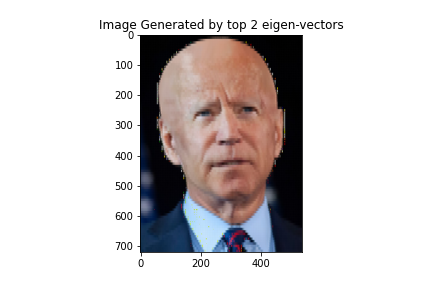
\includegraphics[scale=0.2]{images/q4/joe/joe_2.png}
    \end{subfigure}
    \hfill
    \begin{subfigure}{0.2\linewidth}
        \centering
        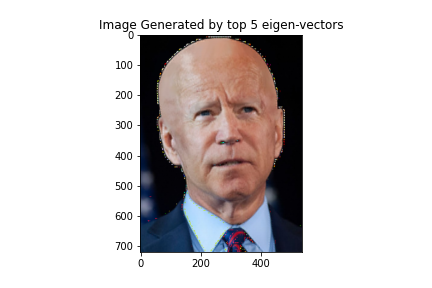
\includegraphics[scale=0.2]{images/q4/joe/joe_5.png}
    \end{subfigure}
    \hfill
    \begin{subfigure}{0.2\linewidth}
        \centering
        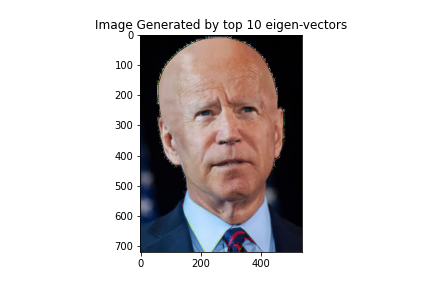
\includegraphics[scale=0.2]{images/q4/joe/joe_10.png}
    \end{subfigure}
    \hfill
    \begin{subfigure}{0.2\linewidth}
        \centering
        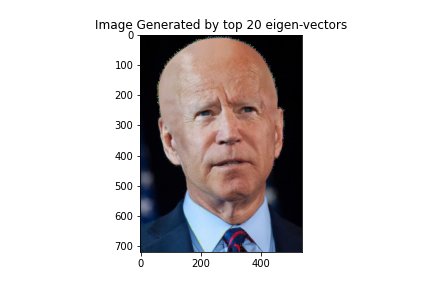
\includegraphics[scale=0.2]{images/q4/joe/joe_20.png}
    \end{subfigure}
    \caption{تصاویر ساخته بازسازی شده با استفاده از تصاویر ویژه}
    \label{joe}
\end{figure}

\section*{سوال پنج}

\subsection*{قسمت الف}

مقادیر بردار‌های ویژه‌ای که الگوریتم \lr{PCA} خروجی می‌دهد، در فایل کد پیوست یعنی \lr{q4.ipynb}
قرار داده شده است. سه مقدار $179.006$، $163.717$ و $141.788$ بزرگترین مقادیر ویژه ارائه شده
هستند.

\subsection*{قسمت ب}

برای حل این سوال فرض کرده‌ایم که یک کرنل از نوع گاوسی داریم. برای پیاده‌سازی این کرنل از تابع

\begin{center}
\lr{\texttt{sklearn.neighbors.KernelDensity()}}
\end{center}

کمک گرفته‌ایم. در قدم بعدی باید مقدار پهنای‌باند را پیدا کنیم. برای پیدا کردن این پارامتر از تابع

\begin{center}
\lr{\texttt{sklearn.model\_selection.GridSearchCV}}
\end{center}

بهره گرفته‌ایم. بازه‌ای که تابع فوق در آن به دنبال پهنای پاند بهینه گشته است بازه $(0,10)$ است.
عددی که توسط این تابع به عنوان پهنای باند بهینه ارائه می‌شود عدد $3.5353$ است.

\subsection*{قسمت ج}

اعداد تولید شده توسط این روش در شکل \ref{eigen_generated} نمایش داده شده است.

\begin{figure}[h]
    \centering
    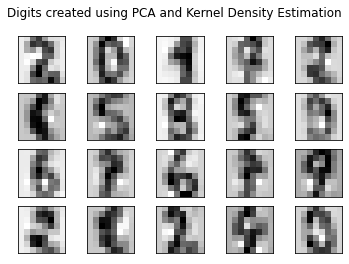
\includegraphics[scale=0.4]{images/q5/eigen_generated.png}
    \caption{اعداد تولید شده در قسمت ج سوال ۵}
    \label{eigen_generated}
\end{figure}

\subsection*{قسمت د}

اعداد تولید شده با حذف قسمت \lr{PCA} در شکل \ref{all_generated} مشاهده می‌شود.
تصاویر تولید شده در این قسمت نسبت به قسمت ج از وضوح بیشتری برخوردار هستند.
این نتیجه قابل توجیه است. چرا که تعداد بردار‌های ویژه ماتریس کوواریانس، در این مسئله
برابر 64 است. این در حالی است که ما در قسمت قبل تنها 15 بردار ویژه را برای تولید
تصاویر استفاده کردیم. بنابراین طبیعی است که تصاویر تولید شده کیفیت کم‌تری داشته باشند.
البته این جمله به این معنا نیست که تصاویر تولید شده در قسمت ج خوانا نیستند.

\begin{figure}[h]
    \centering
    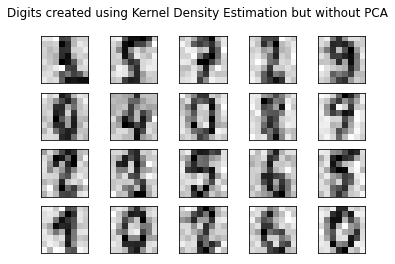
\includegraphics[scale=0.4]{images/q5/all_generated.png}
    \caption{اعداد تولید شده در قسمت د سوال ۵}
    \label{all_generated}
\end{figure}

\section*{سوال ششم}

\subsection*{قسمت ب}

تصاویر بردار‌های ویژه در شکل \ref{eigenfaces} مشاهده می‌شود.

\begin{figure}[h]
    \centering
    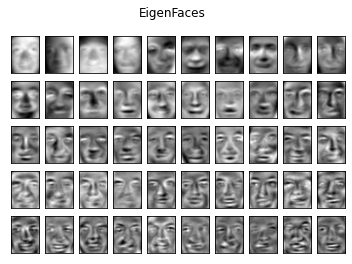
\includegraphics{images/q6/eigenfaces.png}
    \caption{تصویر بردار‌های ویژه در سوال ششم قسمت ب}
    \label{eigenfaces}
\end{figure}

\subsection*{قسمت ج}

تصاویر بردار‌های ویژه در شکل \ref{reproduced_images} مشاهده می‌شود.

\begin{figure}[h]
    \centering
    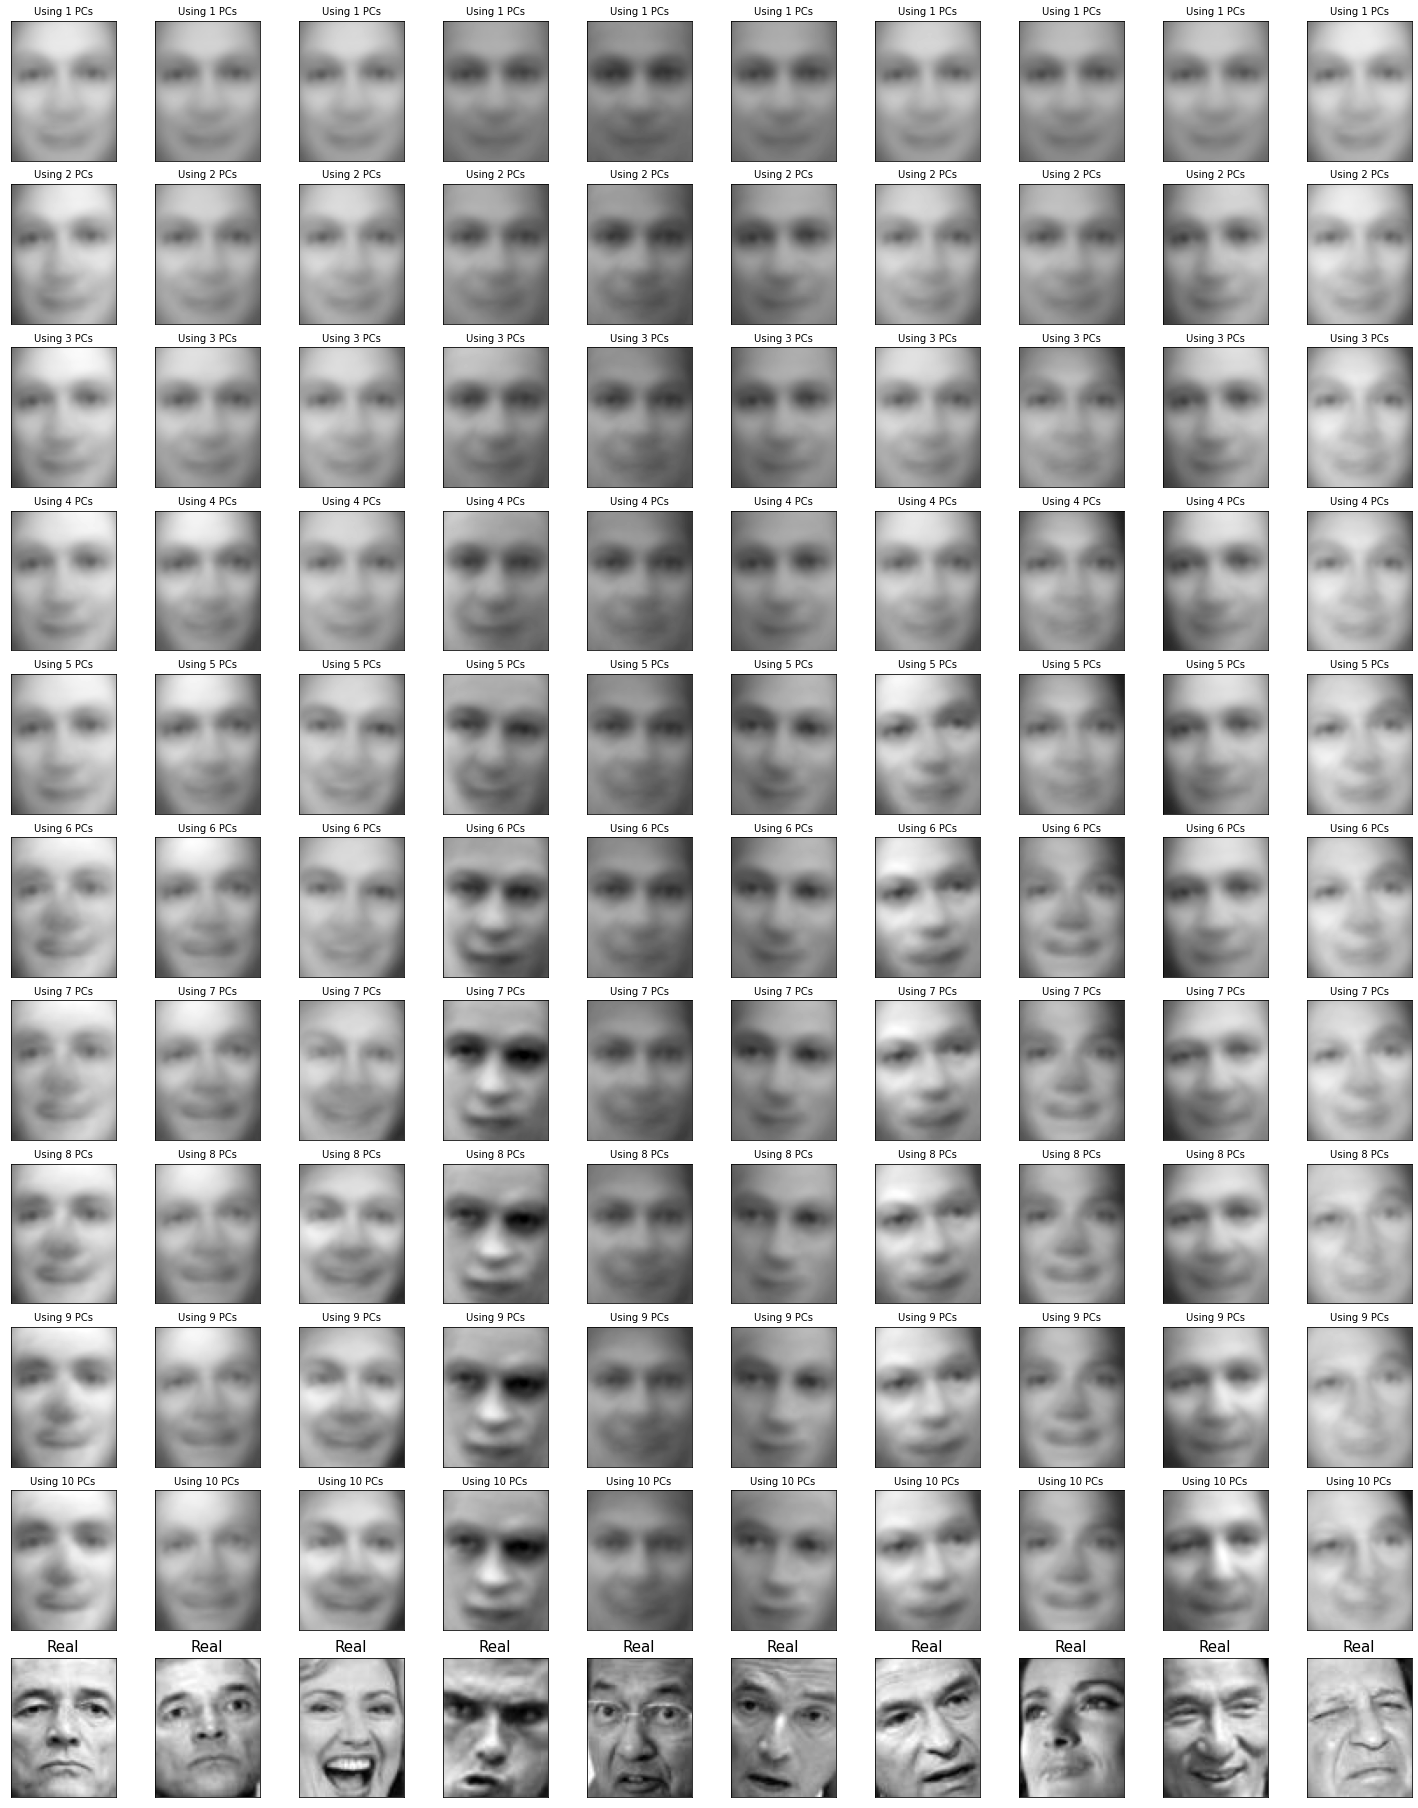
\includegraphics[scale=0.2]{images/q6/reproduced_images.png}
    \caption{تصاویر تولید شده در سوال ششم قسمت ج}
    \label{reproduced_images}
\end{figure}

\subsection*{قسمت د}

نمودار خطا نسبت به \lr{v} به شکل موجود در شکل \ref{q6_all_eigenvectors} حاصل می‌شود.

\begin{figure}[h]
    \centering
    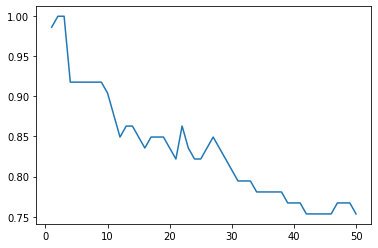
\includegraphics[scale=0.5]{images/q6/result_partd.png}
    \caption{نتایج حاصل شده در قسمت د سوال ۶}
    \label{q6_all_eigenvectors}
\end{figure}

\subsection*{قسمت ه}

نتایج این قسمت در شکل \ref{q6_top_removed_eigenvectors} آورده شده است. همان‌طور که مشاهده می‌شود نتایج در این حالت
نسبت به حالت قبلی بر خلاف انتظار بهتر شده است. دلیلی که برای توجیه این مسئله به نظر می‌رسد این است که مولفه‌های اول
نقش کلیدی در تعیین کلیات تصویر دارند اما این مولفه‌های بعدی هستند که تصاویر را از هم تفکیک می‌کنند. هنگامی که
در دسته‌بندی از مولفه‌های اولیه هم کمک می‌گیریم، این مولفه‌ها تاثیر مولفه‌های بعدی را کم‌تر می‌کنند و در نتیجه تفاوت
چندانی بین تصاویر مشاهده نمی‌شود. برای نشان دادن درستی
این توجیه از شکل \ref{reproduced_images} که تصاویر ساخته شده با استفاده از مولفه‌های اولیه
را نشان می‌دهد کمک می‌گیریم. همان‌طور که مشاهده می‌شود در این تصویر‌ها کلیات تصویر اشخاص با
صرف نظر از جزئیات ساخته شده است. با نگاه کردن به این تصاویر مشخص است که این تصویر یک تصویر چهره است،
اما مشخص نیست که تصویر چهره کدام شخص است. با اضافه شدن بردار‌های ویژه دیگر کم‌کم مشخص می‌شود که چهره ساخته شده
متناظر کدام یک از افراد است.

\begin{figure}[h]
    \centering
    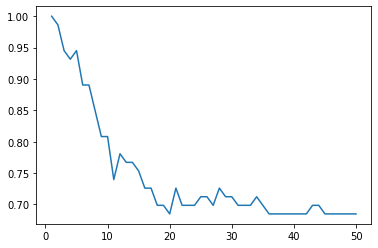
\includegraphics[scale=0.5]{images/q6/result_parte.png}
    \caption{نتایج حاصل شده در قسمت ه سوال ۶}
    \label{q6_top_removed_eigenvectors}
\end{figure}

\subsection*{قسمت ز}

نمودار متناظر این قسمت در شکل \ref{fisher_eigenfaces} آورده شده است.

\begin{figure}[h]
    \centering
    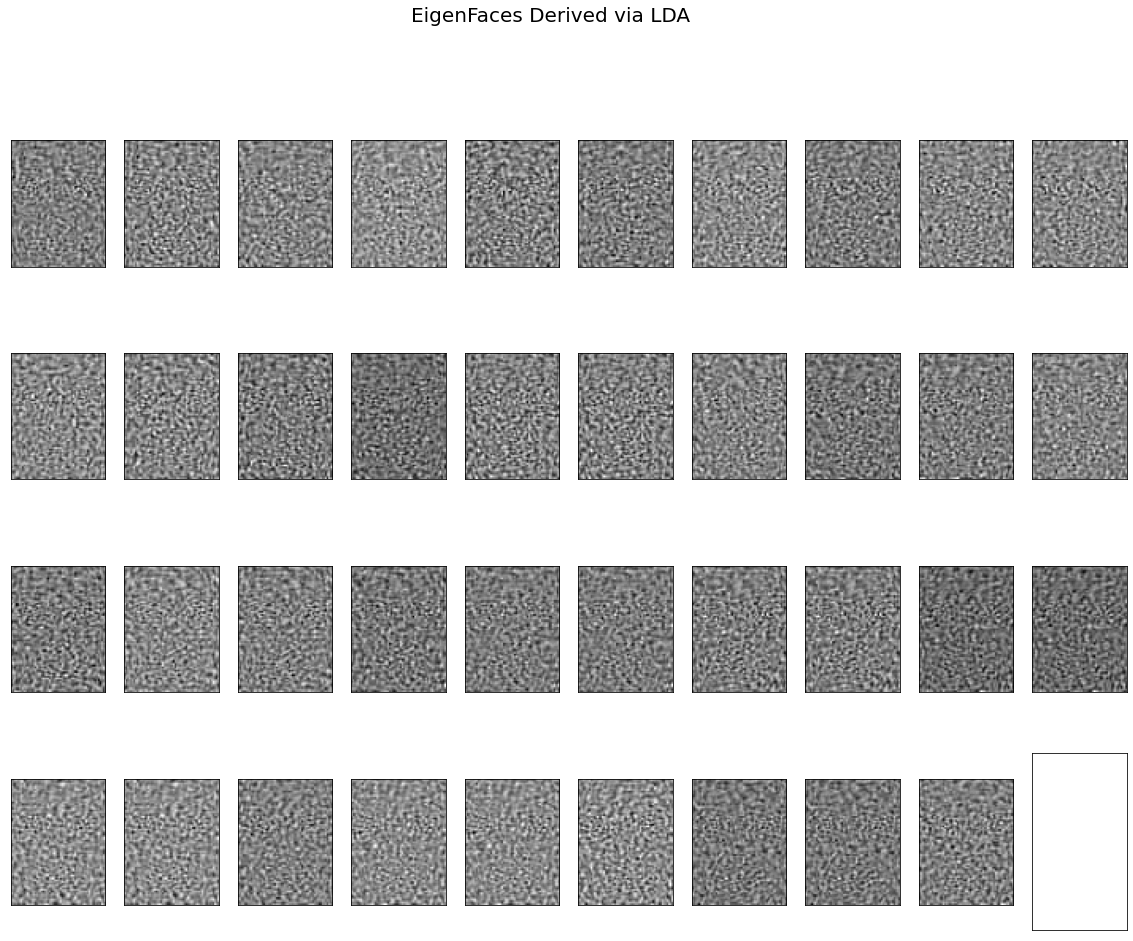
\includegraphics[scale=0.3]{images/q6/partg.png}
    \caption{نتایج حاصل شده در قسمت ز سوال ۶}
    \label{fisher_eigenfaces}
\end{figure}

\subsection*{قسمت ح}

نمودار خطای متناظر این قسمت در شکل \ref{parth_results} مشاهده می‌شود.

\begin{figure}[h]
    \centering
    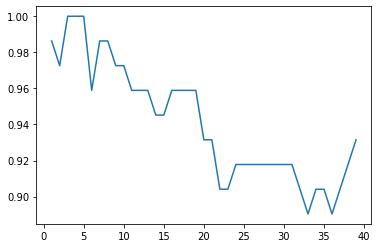
\includegraphics[scale=0.5]{images/q6/parth_results.png}
    \caption{نتایج حاصل شده در قسمت ح سوال ۶}
    \label{parth_results}
\end{figure}

\newpage
\pagebreak

\section*{سوال هفت}

\subsection*{قسمت الف}

روش \lr{Parzen} نسبت به روش \lr{kNN} در مقابله با داده‌های پرت مقاوم‌تر است. در روش \lr{Parzen}
اگر یکی از داده‌ها در فاصله‌ی دوری نسبت به سایر داده‌ها قرار داشته باشد، تنها به بعضی از نقاط اطراف
این داده احتمال نسبت داده می‌شود و بیشتر تابع جرم احتمال در مناطقی قرار می‌گیرد که نقاط در آن جا نزدیک به
هم هستند. اما در روش \lr{kNN} به تمامی اعداد بین آن نقطه پرت و نقاط اصلی احتمال نسبت داده می‌شود.
بدین ترتیب نقاط نزدیک به هم سهم‌کم‌تری در نمودار توزیع تولید شده توسط \lr{kNN} خواهند داشت.

\subsection*{قسمت ب}

اگر $k=1$ باشد، خطا بر روی داده‌های آموزشی برابر صفر خواهد شد. در این حالت در زمان تست بر روی همه داده‌های آموزشی،
هر داده به خودش نگاشت خواهد شد و در نتیجه هیچ داده‌ای برچسب اشتباه نمی‌خورد.

اگر $k=3$ نتایج بستگی به دیتاست و تعداد کلاس‌های دسته‌بندی دارد و به طور قطعی نمی‌توان نظر داد.

اگر $k=n$ باشد، در این صورت همواره تمامی داده‌های تست به برچسبی نگاشت خواهند شد که بیشترین تعداد را در داده آموزشی
دارد در نتیجه در این حالت خطا کوچکتر مساوی $\frac{1}{c}$ خواهد بود. $c$ تعداد کلاس‌های آموزشی است.

\subsection*{قسمت ج}

در داده‌هایی که در شکل \ref{distances} نشان داده شده‌اند، فرض کنیم بخواهیم از دسته‌بند \lr{kNN} با مقدار
$k=1$ برای دسته‌بندی داده‌ها استفاده کنیم. داده‌های آموزشی با رنگ قرمز و آبی (که معرف کلاس‌های مختلف است) و داده‌های
تست با رنگ خاکستری مشخص شده‌اند.

در هنگام دسته‌بندی اگر از فاصله اقلیدسی استفاده کنیم، هر دو داده \lr{‌‌B} و \lr{D} به عنوان کلاس قرمز دسته‌بندی می‌شوند.
اما اگر از فاصله کسینوسی استفاده کنیم، برای داده \lr{B} برچسب آبی و برای داده \lr{D} برچسب قرمز زده می‌شود.

\begin{figure}[h]
    \centering
    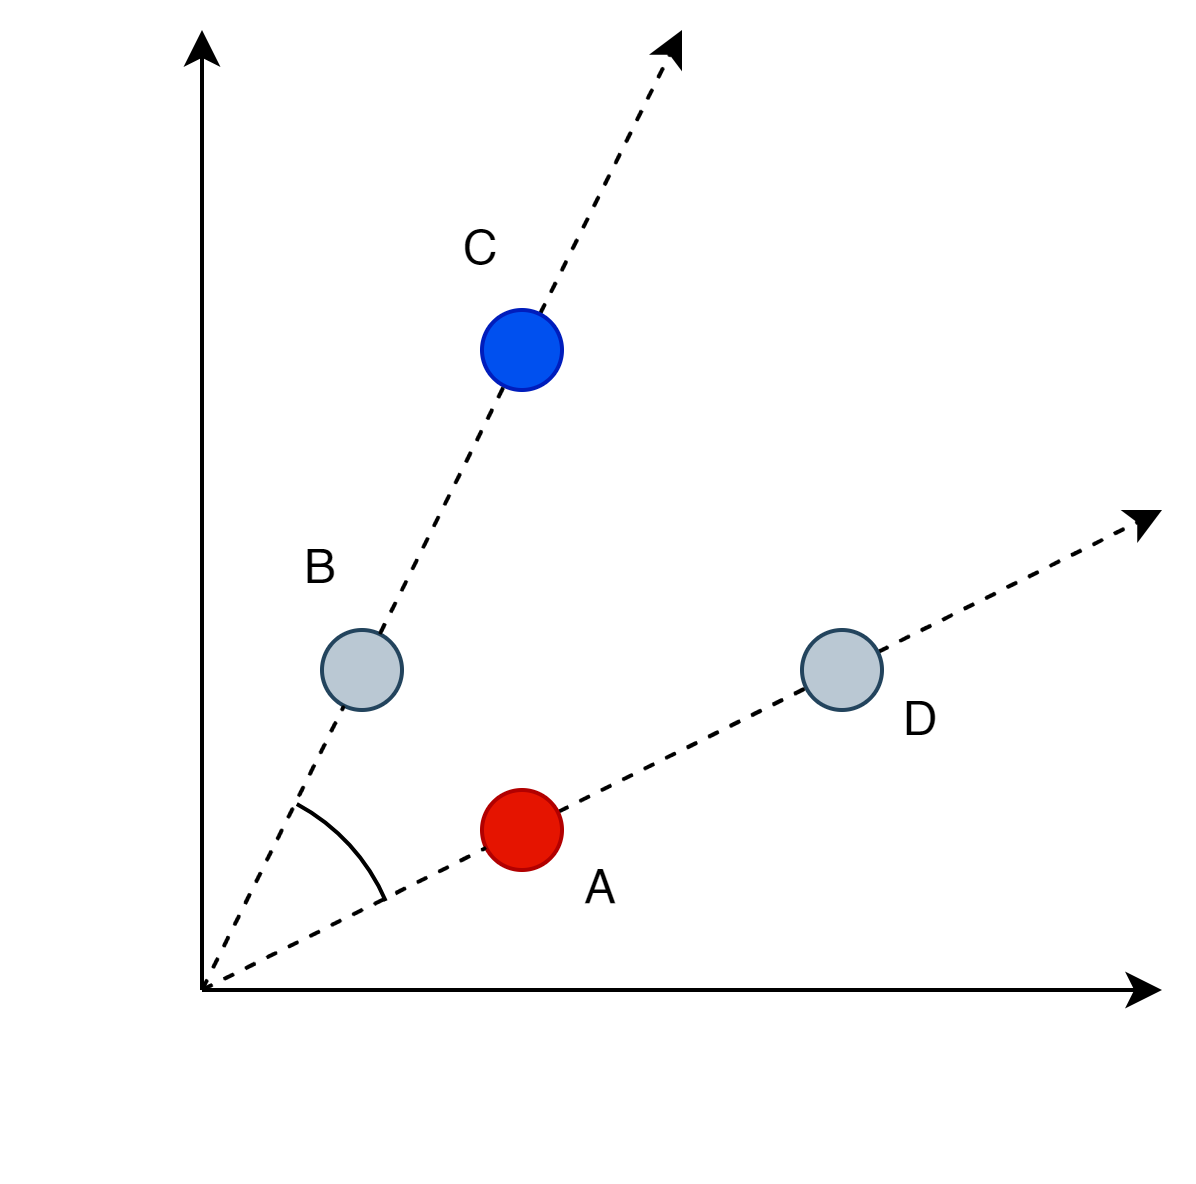
\includegraphics[scale=0.4]{images/q7/partc.png}
    \caption{شکل مربوط به سوال ۷ قسمت ج}
    \label{distances}
\end{figure}

\subsection*{قسمت د}

اگر تعداد داده‌های آموزشی بی‌نهایت باشد در این صورت تخمین توزیع انجام شده در روش \lr{Parzen}
با هر مقدار اندازه پنجره و روش \lr{kNN} با مقدار $k=\infty$ به یک نتیجه منتهی خواهد شد.

\subsection*{قسمت ه}

خیر این مسئله امکان ندارد. در روش \lr{PCA} ابتدا ماتریس \lr{Scatter} محاسبه شده و از روی آن
بردار‌های ویژه به دست می‌آید. از آن جا که ابعاد ماتریس \lr{Scatter} به اندازه ابعاد داده‌ها است،
بنابراین حداکثر به همان اندازه می‌تواند بردار ویژه داشته باشد.

\subsection*{قسمت و}

می‌دانیم با استفاده از \lr{PCA} می‌توانیم بردار‌های ویژه که بردار‌های اصلی سازنده تصویر هستند را به دست آوریم
اگر از تمامی بردار‌های ویژه برای بازسازی تصویر کمک بگیریم، تصویر اولیه عینا به دست می‌آید اما اگر تنها از
بردار‌های ويژه مهم که متناظر مقادیر ویژه بزرگ هستند استفاده کنیم، در این صورت تصویر اولیه بدون جزئیات
به دست خواهد آمد. نبود جزئیات در اکثر موارد یک نقطه ضعف به حساب می‌آید اما درتصویری که دارای نویز است،
نبود جزئیات به معنای کم‌بودن نویز خواهد بود و در نتیجه می‌توانیم از این شیوه برای کم‌کردن نویز در تصویر استفاده کنیم.

\subsection*{قسمت ز}

در روش \lr{PCA} بردار‌های ویژه داده‌ها به دست آمده و سپس در ادامه با استفاده از این بردار‌های ویژه
ابعاد داده‌ها را کاهش می‌دهند. اگر ابعاد داده‌ها زیاد باشد در این صورت به دست آوردن بردار‌های ویژه از
ماتریس \lr{Scatter} کار دشواری خواهد بود. برای کم‌کردن حجم محاسبات به دست آوردن بردار‌های ویژه
راه‌حل‌های زیر به ذهن می‌رسد.

\begin{itemize}
    \item تبدیل چند پیکسل کنار هم به یک پیکسل. برای مثال می‌توان میانگین چند پیکسل کنار هم را محاسبه کرده
    و عدد حاصل را به جای این پیکسل‌ها استفاده کرد.
    \item تبدیل تصویر بزرگ به چند تصویر با ابعاد کوچک‌تر و انجام \lr{PCA} بر روی تصاویر کوچک.
\end{itemize}

\end{document}